\chapter{測地線、一様加速、ニュートン極限}

当面の問題は重力である。より正確には、地球表面近くの小さな実験室における場のような、ほぼ一様な重力場を記述する時空計量を求めたい。その計量への最短経路は、実は直接的なものではない。まず三つの幾何学的な考え方を操作可能な形にしなければならない。すなわち、共変微分、平行移動、そして測地線運動である。

これらの考え方は互いに依存している。共変微分は、隣接する点におけるベクトルをどのように比較するかを教える。平行移動は、ベクトルを回転させずに運ぶ方法を教える。測地線は、運ばれるベクトルが経路自身の接ベクトルであるときに得られる。経路が空間内ではなく時空内にあるとすれば、同じ測地線方程式が自由落下粒子の運動方程式となる。

講義の後半では、次に印象的な展開がなされる。我々は平坦なミンコフスキー時空にとどまるが、それを剛体加速する観測者族に適合した座標で記述する。それらの座標では、計量は重力的に見える。ある観測者の近くでは、一様な場のポテンシャルを再現し、その測地線はニュートン方程式
\begin{equation}
\frac{d^2y}{d\tau^2}=-g.
\end{equation}
に従う。これは等価原理を計算として書き表したものである。

\section{共変微分の再確認}

選ばれた点\(P\)において、できるだけデカルト的になるような座標を選ぶことができる。講義では当初ガウス正規座標という語を用い、直ちにそれに限定を加える。名称よりも局所的な条件の方が重要である。
\begin{equation}
g_{mn}(P)=\delta_{mn},
\qquad
\partial_r g_{mn}(P)=0.
\label{eq:l4-normal-point}
\end{equation}
これらは一点における正規座標である。有限な近傍でデカルト的であり続ける必要はなく、軸を回転させることができるため、そのような枠は多数存在する。

計量は微分作用素と整合している。
\begin{equation}
\nabla_r g_{mn}=0,
\qquad
\nabla_r g^{mn}=0.
\label{eq:l4-metric-compatibility}
\end{equation}
余ベクトル\(V_s\)に対して、共変微分は
\begin{equation}
\nabla_r V_s
=
\partial_r V_s-\Gamma^p{}_{rs}V_p.
\label{eq:l4-covector-derivative}
\end{equation}
である。接続係数は
\begin{equation}
\Gamma^p{}_{rs}
=
\frac{1}{2}g^{pn}
\left(
\partial_s g_{nr}
+\partial_r g_{ns}
-\partial_n g_{rs}
\right).
\label{eq:l4-christoffel}
\end{equation}
である。この式が黒板に書かれる間にいくつかの添字が修正される。式\eqref{eq:l4-christoffel}が完成した関係式である。\(r\)と\(s\)について対称であり、捩れのないレヴィ・チヴィタ接続に期待されるとおりである。

\begin{figure}[htbp]
\centering
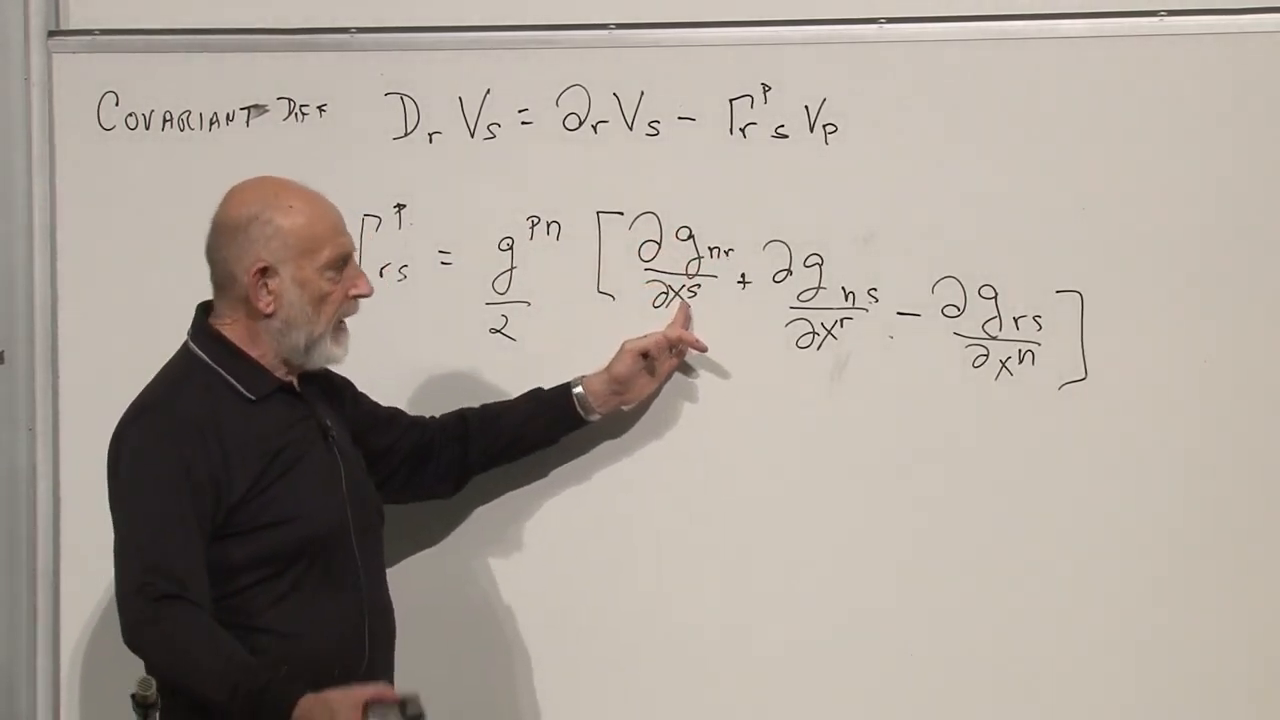
\includegraphics[width=0.92\textwidth]{lecture_04_figure_01.png}
\caption{余ベクトルの微分と完成したクリストッフェル記号の公式。}
\end{figure}

クリストッフェル記号は計量の一階微分から作られるため、座標\eqref{eq:l4-normal-point}において\(P\)で消える。しかし、基礎となる空間が平坦であっても、あらゆる座標系で消えるわけではない。したがって\(\Gamma^p{}_{rs}\)はテンソルではない。この非テンソル的な性質こそ、後に、加速する観測者が慣性観測者には見えない重力を記述できるようにするものである。

\subsection{ベクトルの添字を上げる}

ベクトルの対応する微分は、暗記すべき別個の規則として導入されるのではない。それは計量から従う。まず
\begin{equation}
V^n=g^{np}V_p.
\end{equation}
から始める。すると
\begin{align}
\nabla_m V^n
&=\nabla_m\!\left(g^{np}V_p\right) \\
&=(\nabla_m g^{np})V_p+g^{np}\nabla_m V_p \\
&=g^{np}\left(\partial_mV_p-\Gamma^r{}_{mp}V_r\right),
\end{align}
となり、ここで計量整合性により第一項が消えた。添字を整理すると
\begin{equation}
\nabla_m V^n
=
\partial_m V^n+\Gamma^n{}_{mr}V^r.
\label{eq:l4-vector-derivative}
\end{equation}
が得られる。

\begin{figure}[htbp]
\centering
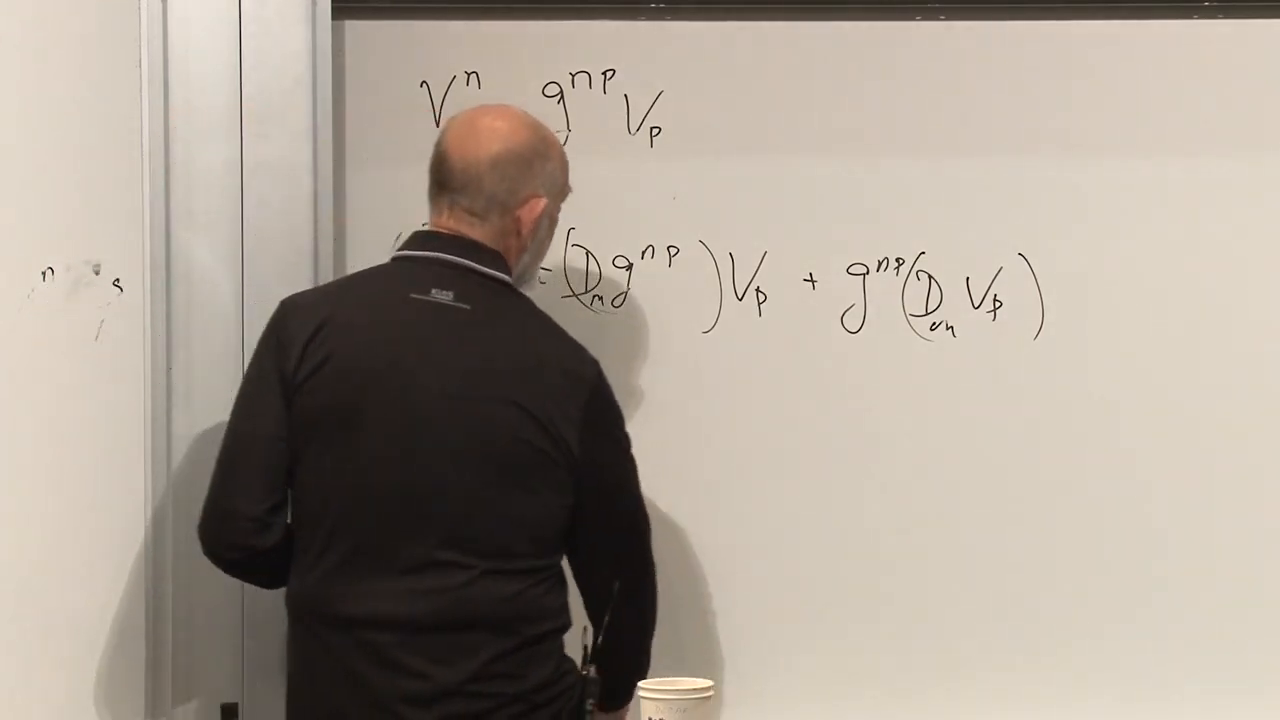
\includegraphics[width=0.90\textwidth]{lecture_04_figure_02.png}
\caption{微分する前に逆計量で添字を上げる。}
\end{figure}

\begin{figure}[htbp]
\centering
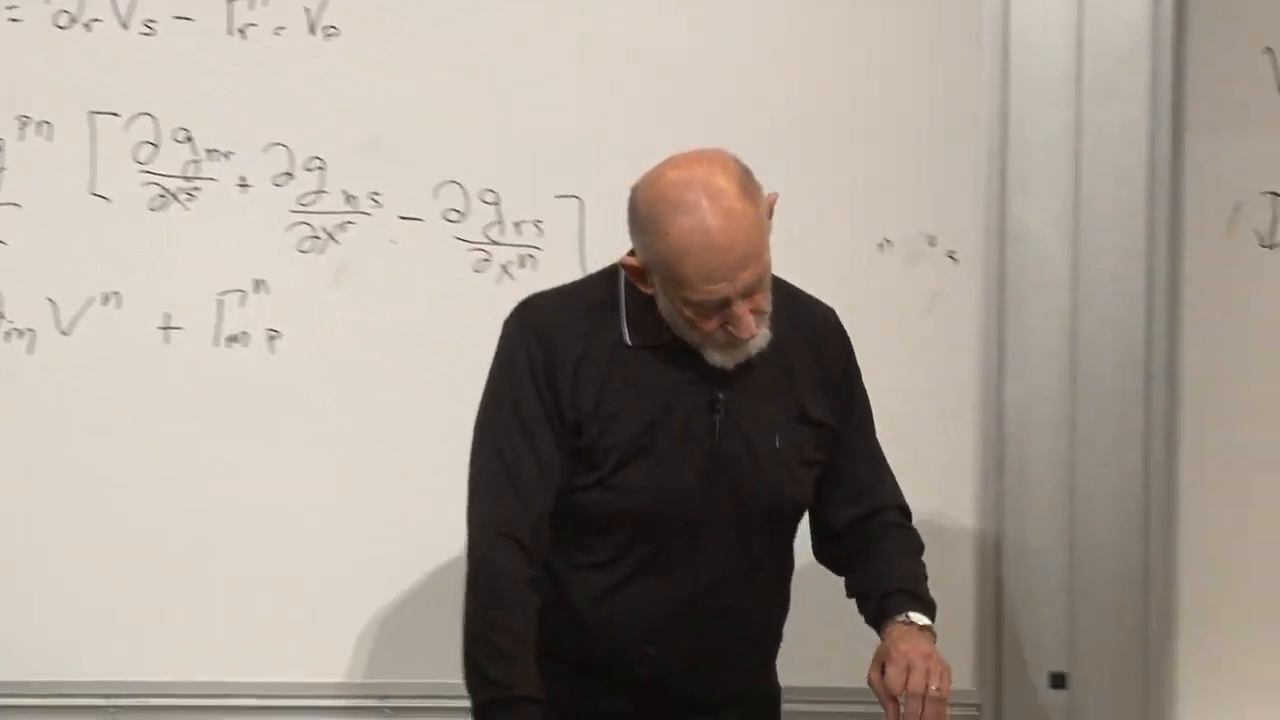
\includegraphics[width=0.90\textwidth]{lecture_04_figure_03.png}
\caption{計量整合性と積の法則から現れる上付き添字の微分。}
\end{figure}

したがって添字の文法は単純である。
\begin{equation}
\boxed{
\begin{aligned}
\text{lower index:}&\quad -\Gamma,\\
\text{upper index:}&\quad +\Gamma.
\end{aligned}}
\end{equation}
高階のテンソルでは、各添字に対して一つの接続項が現れ、その符号はその添字が下付きか上付きかによって決まる。

\subsection{用語に関する問い}

上で言及した最良の座標とは正確には何か。それらは特別な大域座標系として主張されているのではない。一つの選ばれた点において、計量をその平坦な形に等しくし、その一階微分を消すのである。軸を回転させれば、別の同様に良い枠が得られる。そのような枠で導かれた幾何学的な命題は、最終的な対象がテンソルであるため、その向きに依存しない。

\section{曲線に沿った平行移動}

ベクトル\(V^n\)が曲線に沿って運ばれるとする。微小変位\(dx^m\)にわたるその共変変化は
\begin{align}
\delta V^n
&=(\nabla_mV^n)\,dx^m \\
&=\partial_mV^n\,dx^m
+\Gamma^n{}_{mr}V^r\,dx^m \\
&=dV^n+\Gamma^n{}_{mr}V^r\,dx^m.
\label{eq:l4-covariant-differential}
\end{align}
である。

\begin{figure}[htbp]
\centering
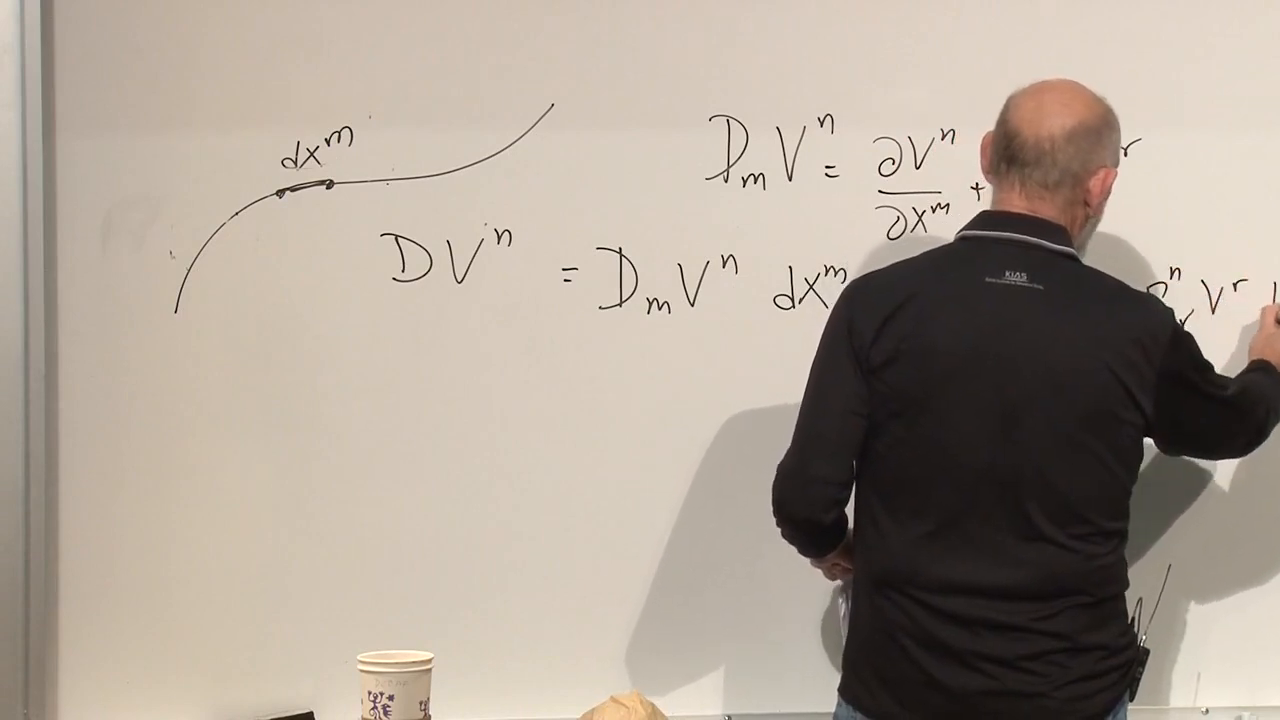
\includegraphics[width=0.92\textwidth]{lecture_04_figure_04.png}
\caption{曲線に沿った通常の成分変化と接続による補正。}
\end{figure}

この共変変化が消えるとき、ベクトルは平行移動される。
\begin{equation}
\boxed{
dV^n+\Gamma^n{}_{mr}V^r\,dx^m=0.
}
\label{eq:l4-parallel-transport}
\end{equation}
操作上は、曲線の各点で正規枠を立てることを想像すればよい。その局所枠において、運ばれるベクトルは回転しないことが要求される。次に微小距離だけ移動し、次の正規枠を立て、これを繰り返す。

\begin{figure}[htbp]
\centering
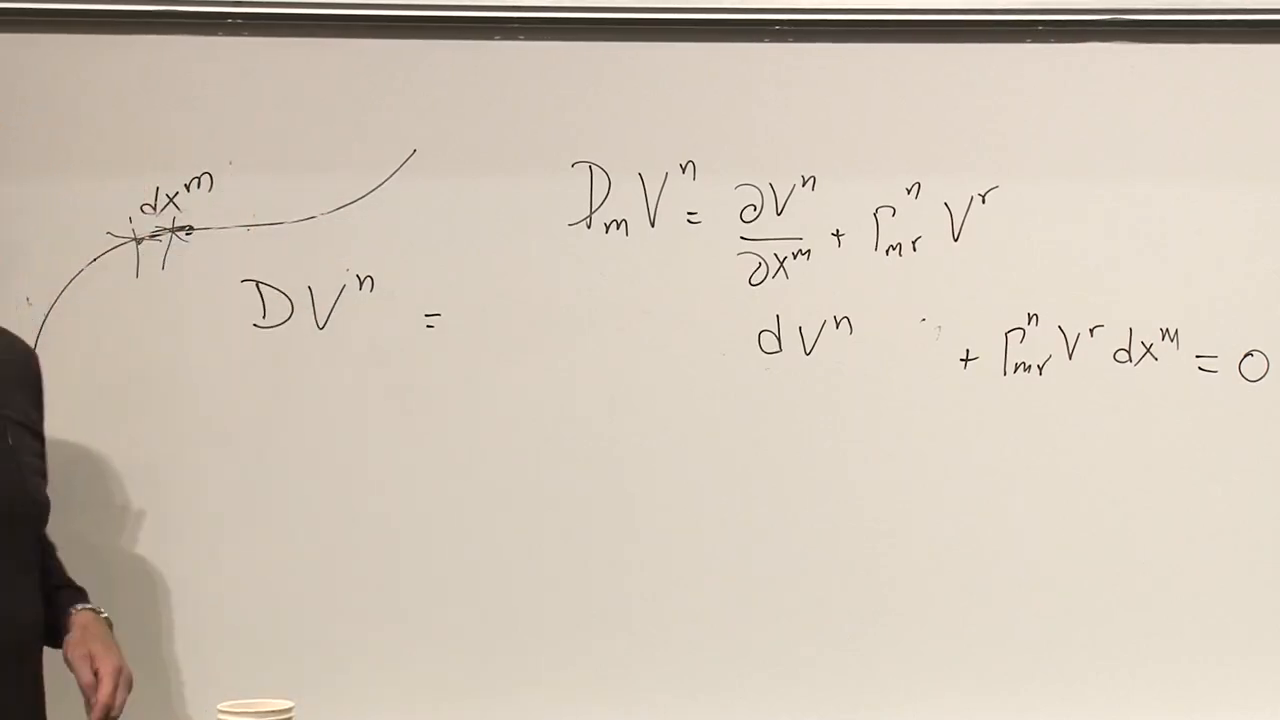
\includegraphics[width=0.92\textwidth]{lecture_04_figure_05.png}
\caption{平行移動の方程式の明確な板書状態。}
\end{figure}

それぞれの一時的な正規枠の向きは物理の一部ではない。比較を行う前にそれを回転させてもよい。重要なのは、共変的な記述\eqref{eq:l4-parallel-transport}がその任意の選択に依存しないことである。

\subsection{経路依存性と曲率}

曲がった空間では、平行移動は経路に依存する。同じ初期点で同じベクトルから始め、二つの異なる経路に沿って同じ終点までそれを移動させる。一般に、最終的なベクトルは異なる。ベクトルを閉じたループに沿って一周させると、回転した状態で戻ってくることがある。その不一致がホロノミーであり、曲率の直接的な徴候である。

\begin{figure}[htbp]
\centering
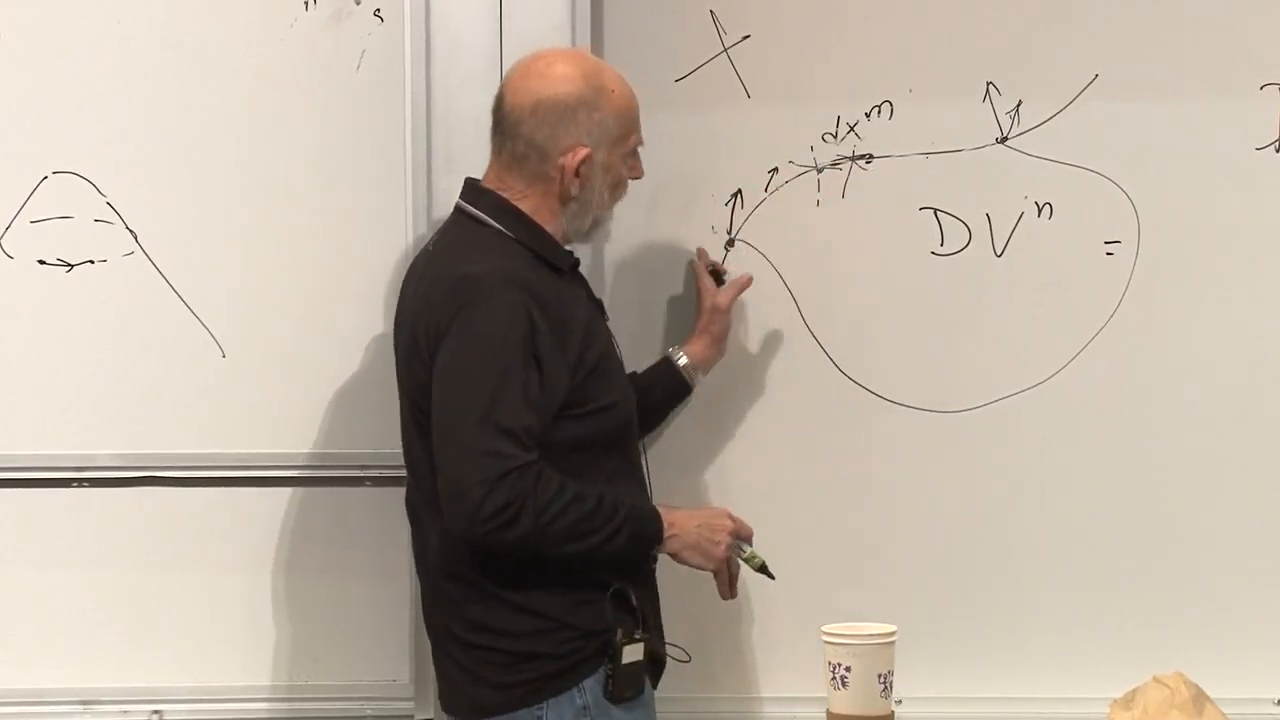
\includegraphics[width=0.90\textwidth]{lecture_04_figure_06.png}
\caption{曲面上の二つの経路は、ベクトルを同じ最終的な向きに移動させる必要はない。}
\end{figure}

円錐は有用な例を与える。その先端から離れたところでは、円錐を切り開いて平らに広げることができる。それにもかかわらず、先端を囲むループの周りで平行移動させると、ベクトルは角度欠損だけ回転して戻ってくる。先端が丸められていれば、曲率は有限であり小さな領域に広がっている。完全に鋭ければ、理想化によって曲率は先端に集中する。

\begin{figure}[htbp]
\centering
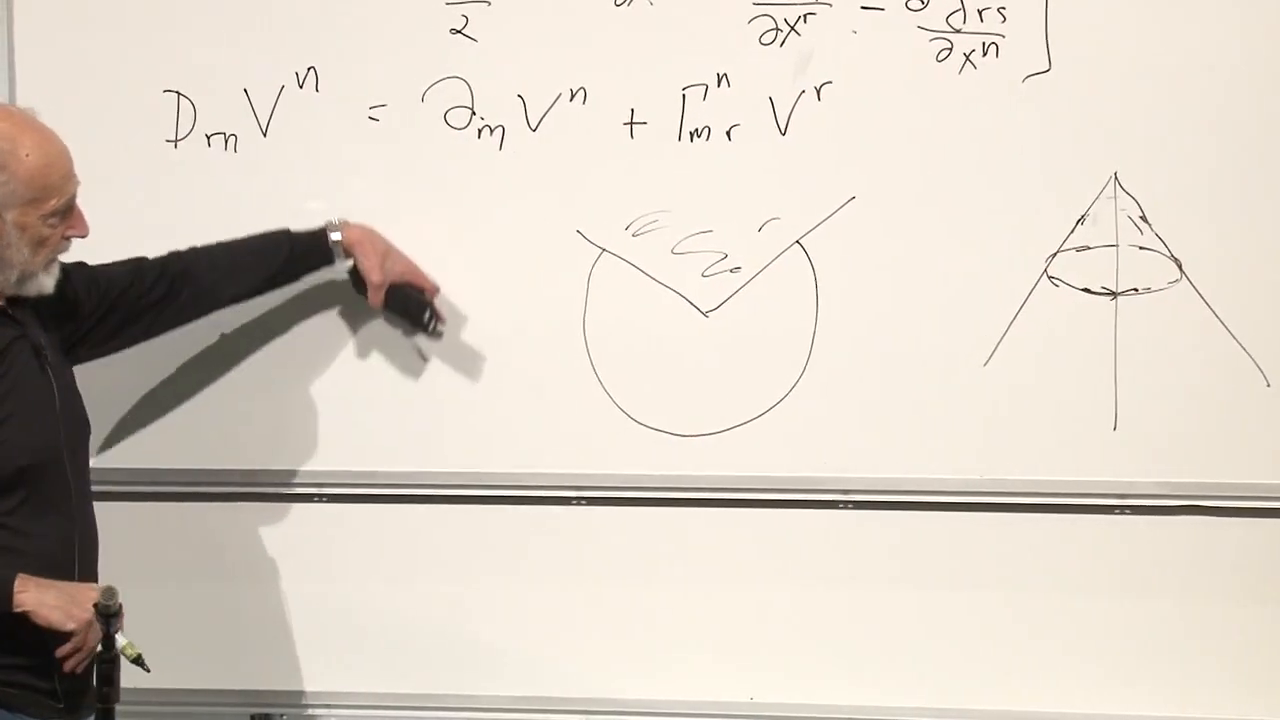
\includegraphics[width=0.90\textwidth]{lecture_04_figure_07.png}
\caption{円錐上の円運動とその切り開いた平面表示。}
\end{figure}

\subsection{移動されたベクトルに関する問い}

\paragraph{ベクトルは至る所で定義されなければならないか。}
いいえ。一点における単一のベクトルから始め、選んだ曲線に沿ってのみ\eqref{eq:l4-parallel-transport}を解いてもよい。完全なベクトル場は任意である。ある領域上で場が定義されている場合、それは一つの方向に沿って共変的に一定であっても、別の方向に沿ってはそうでないことがある。

\paragraph{その長さは保存されるか。}
はい。\(V^2=g_{mn}V^mV^n\)とおく。曲線に沿って、
\begin{align}
\frac{D}{d\lambda}\left(g_{mn}V^mV^n\right)
&=
\frac{Dg_{mn}}{d\lambda}V^mV^n
+2g_{mn}V^m\frac{DV^n}{d\lambda}\\
&=0.
\end{align}
計量整合性が第一項を消し、平行移動が第二項を消す。したがって、平行移動されたベクトルの長さと相互の角度は保存される。

\paragraph{すべての曲線の接ベクトルは平行移動されるか。}
いいえ。この問いは測地線へ直接つながる。円錐の周りの円経路の接ベクトルは絶えず向きを変える。円錐を切り開いて得られる直線の接ベクトルはそうではない。局所的にまっすぐなのは第二の経路のみである。

\section{測地線：単に最短であるよりも最もまっすぐ}

測地線には二つの関連する記述がある。大域的には、それは長さまたは固有時間の汎関数の停留経路である。局所的には、それは可能な限り最もまっすぐな経路である。停留という語は重要である。幾何と端点に応じて、その経路は唯一の大域的最小値である必要はない。ローレンツ時空では、時間的測地線は正の距離を最小化するのではなく、局所的に固有時間を最大化する。

ここで必要なのは局所的な記述である。曲がった地形の上を、ハンドルをまっすぐに保ったまま小型車で走らせると、地形が曲がる尺度に比べて車が小さければ、その車は測地線を描く。それは埋め込み空間の中でまっすぐに見える必要はない。表面上で利用可能な幾何に従ってまっすぐなのである。

\begin{figure}[htbp]
\centering
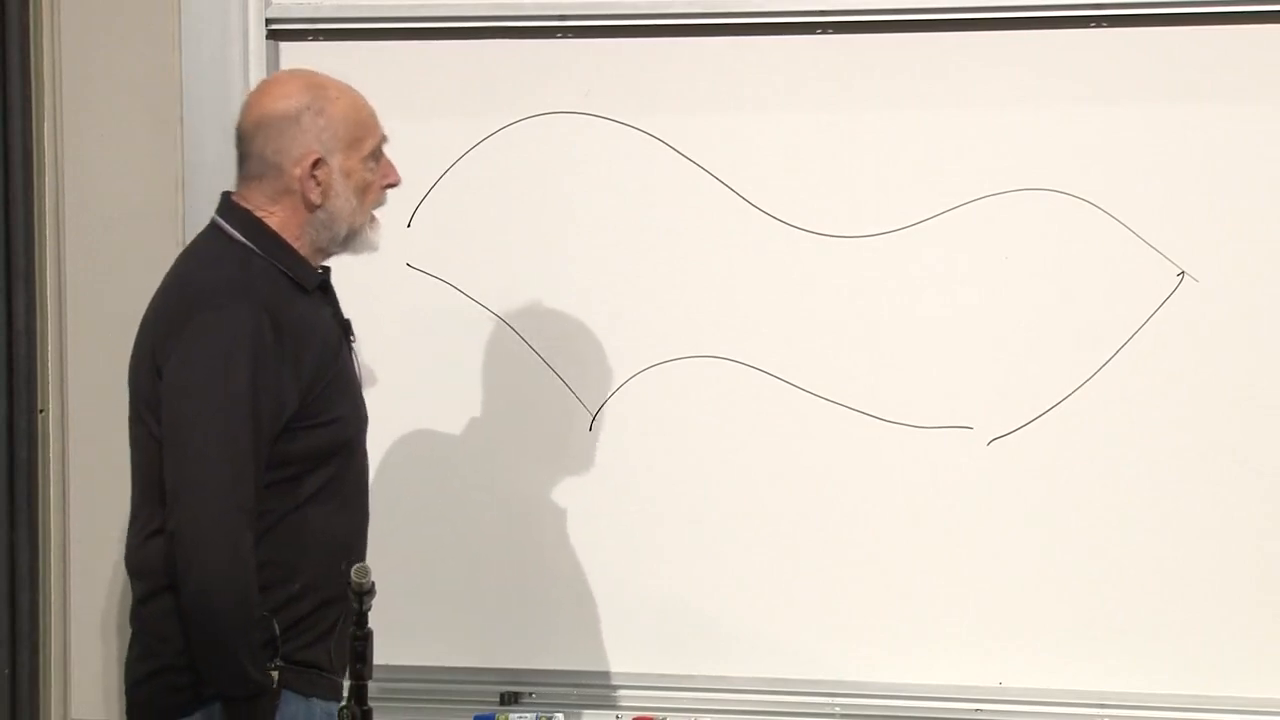
\includegraphics[width=0.90\textwidth]{lecture_04_figure_08.png}
\caption{曲面上に内在的に描かれた経路。最もまっすぐな経路の定義の準備。}
\end{figure}

\subsection{接ベクトル}

曲線を\(x^m(s)\)とし、弧長を
\begin{equation}
ds^2=g_{mn}\,dx^m dx^n.
\end{equation}
とする。単位接ベクトルは
\begin{equation}
t^m=\frac{dx^m}{ds}.
\label{eq:l4-unit-tangent}
\end{equation}
である。幾何学的には、近くの二点を取り、それらの間の変位ベクトルを作り、その間隔で割り、点を一致させる。

\begin{figure}[htbp]
\centering
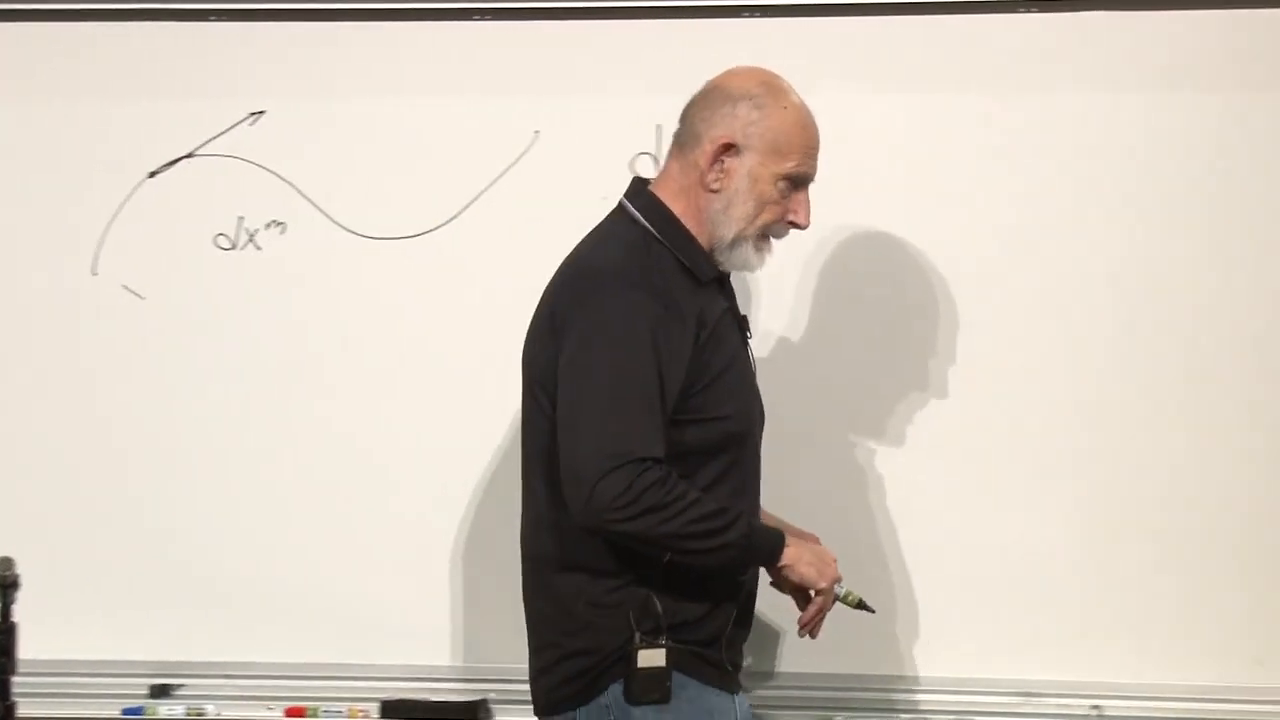
\includegraphics[width=0.90\textwidth]{lecture_04_figure_09.png}
\caption{曲線に沿った極限の変位としての接方向。}
\end{figure}

\begin{figure}[htbp]
\centering
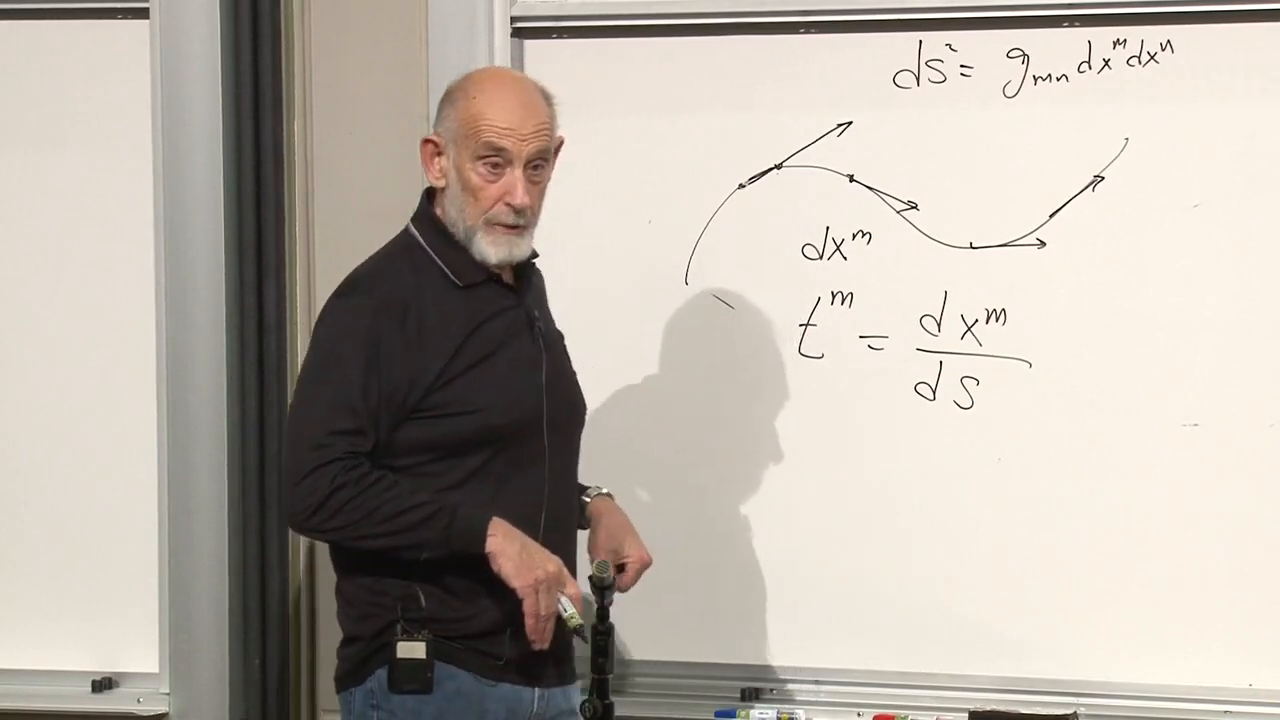
\includegraphics[width=0.90\textwidth]{lecture_04_figure_10.png}
\caption{線素と単位接ベクトル\(t^m=dx^m/ds\)。}
\end{figure}

測地線とは、その接ベクトルがそれ自身に沿って平行移動される曲線である：
\begin{equation}
dt^n+\Gamma^n{}_{mr}t^r\,dx^m=0.
\end{equation}
\(ds\)で割り、\(dx^m/ds=t^m\)を用いると：
\begin{equation}
\frac{dt^n}{ds}
=
-\Gamma^n{}_{mr}t^m t^r.
\end{equation}
最後に\(t^n=dx^n/ds\)を代入すると：
\begin{equation}
\boxed{
\frac{d^2x^n}{ds^2}
+\Gamma^n{}_{mr}
\frac{dx^m}{ds}
\frac{dx^r}{ds}
=0.
}
\label{eq:l4-geodesic}
\end{equation}

\begin{figure}[htbp]
\centering
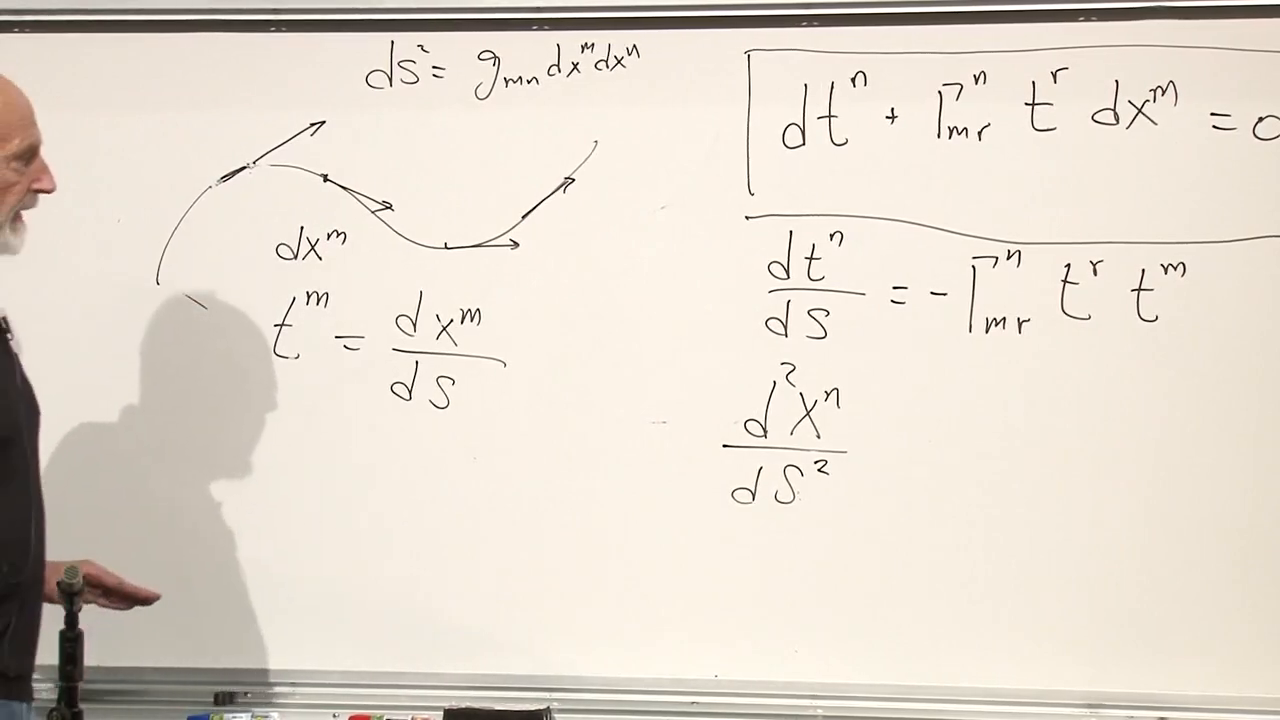
\includegraphics[width=0.94\textwidth]{lecture_04_figure_11.png}
\caption{接ベクトルの移動法則と二階の測地線方程式。}
\end{figure}

式\eqref{eq:l4-geodesic}はすでにニュートン力学に似ている。\(s\)を適切な時間パラメータに置き換えれば、第一項は加速度である。すると接続項は、計量のみによって決まる単位質量あたりの力のように働く。一般相対性理論ではこの類推は文字通りになる。自由粒子は時空の測地線に従い、ニュートンが重力加速度と呼んだものは接続を通じて現れる。

\section{リーマン距離から時空の固有時間へ}

議論はここで曲がった空間から時空へ移る。慣性直交座標では、近接する事象間の固有時間は
\begin{equation}
d\tau^2
=dt^2-dx^2-dy^2-dz^2.
\label{eq:l4-proper-time}
\end{equation}
である。講義では
\begin{equation}
d\tau^2=-g_{\mu\nu}\,dx^\mu dx^\nu
\label{eq:l4-lecture-sign}
\end{equation}
を用い、
\begin{equation}
g_{\mu\nu}
=
\eta_{\mu\nu}
=
\begin{pmatrix}
-1&0&0&0\\
0&1&0&0\\
0&0&1&0\\
0&0&0&1
\end{pmatrix}.
\label{eq:l4-eta}
\end{equation}
とする。したがって、\eqref{eq:l4-lecture-sign}における外側の負号は、選ばれた mostly-plus 計量を\eqref{eq:l4-proper-time}に変換する。座標は
\begin{equation}
\begin{aligned}
x^\mu&=(t,x,y,z),\\
x^0&=t,\quad x^1=x,\\
x^2&=y,\quad x^3=z.
\end{aligned}
\end{equation}

\begin{figure}[htbp]
\centering
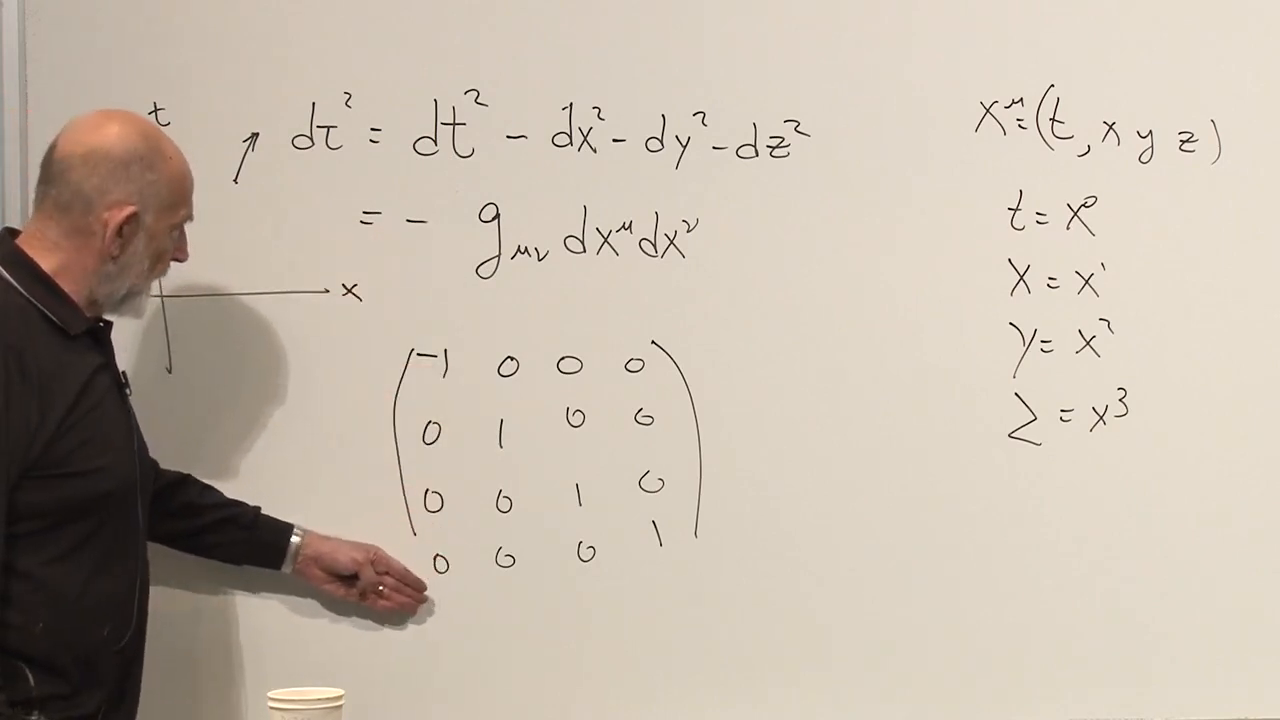
\includegraphics[width=0.94\textwidth]{lecture_04_figure_12.png}
\caption{固有時、時空座標、および mostly-plus ミンコフスキー計量。}
\end{figure}

符号数が不変な情報である。すなわち、1つの固有値が時間に対応する符号を持ち、3つが空間に対応する符号を持つ。計量全体に \(-1\) を掛け、すべての規約を整合的に調整すれば、同様に一般的な mostly-minus 規約が得られる。物理的なものはこの全体的な選択に依存しない。

講義では、他の不定符号数を持つ空間が検討されたことがあるかと問われる。数学的には、多くの符号数を持つ擬リーマン幾何学は十分に確立されている。物理的な要点はより限定的である。観測される相対論的時空はローレンツ的であり、時間的方向を1つ持つ。追加の時間的方向は因果構造を根本的に変えてしまい、ここで議論されている物理を記述しない。

\begin{figure}[htbp]
\centering
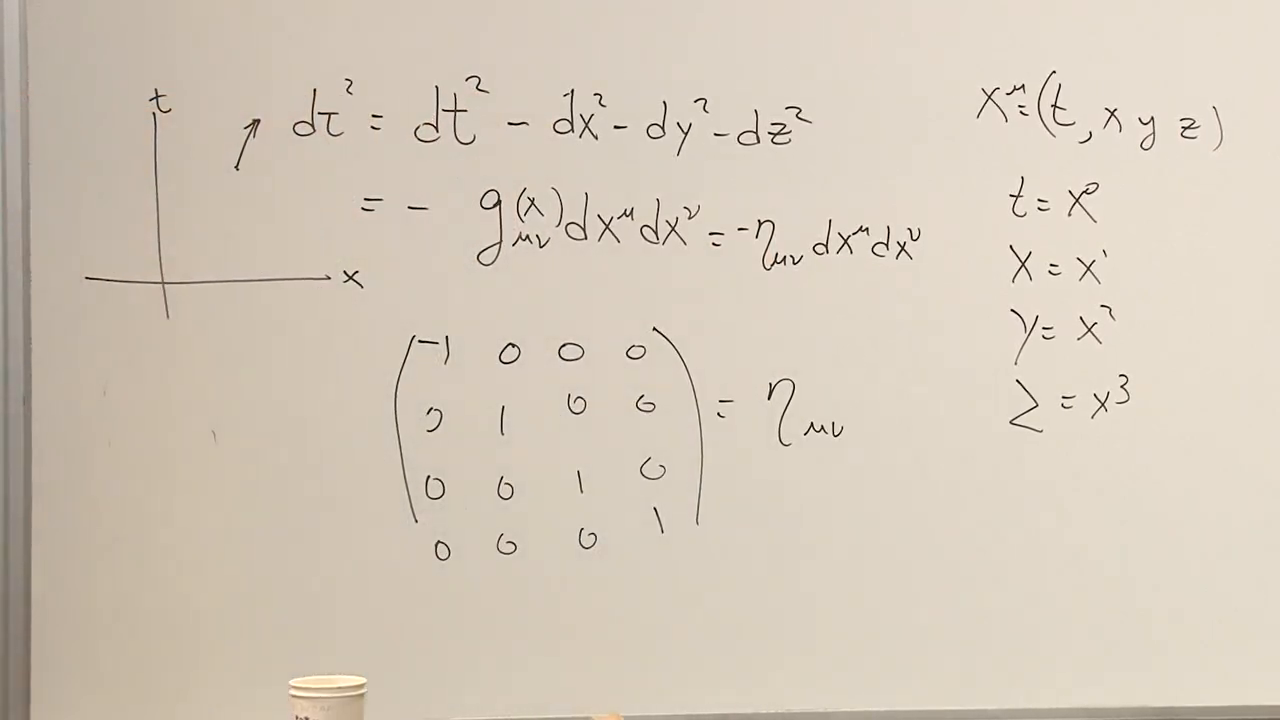
\includegraphics[width=0.94\textwidth]{lecture_04_figure_13.png}
\caption{平坦計量を \(\eta_{\mu\nu}\) で表す前に、符号規約を確認する。}
\end{figure}

平坦時空とは、計量の成分がすべての座標系で \(\eta_{\mu\nu}\) のように見えなければならないという意味ではない。そのように見える座標が存在するという意味である。曲線座標や加速座標では、リーマンテンソルがゼロであっても、成分が位置に依存して変化しうる。

\section{なぜ等しい座標加速度は剛体ではないのか}

加速するエレベーターに付随する座標が欲しい。最初のアイデアは、固定された間隔に観測者を並べ、全員に同じ座標加速度を与えることである。相対性理論は、その素朴な構成が剛体のままでいることを妨げる。

\begin{figure}[htbp]
\centering
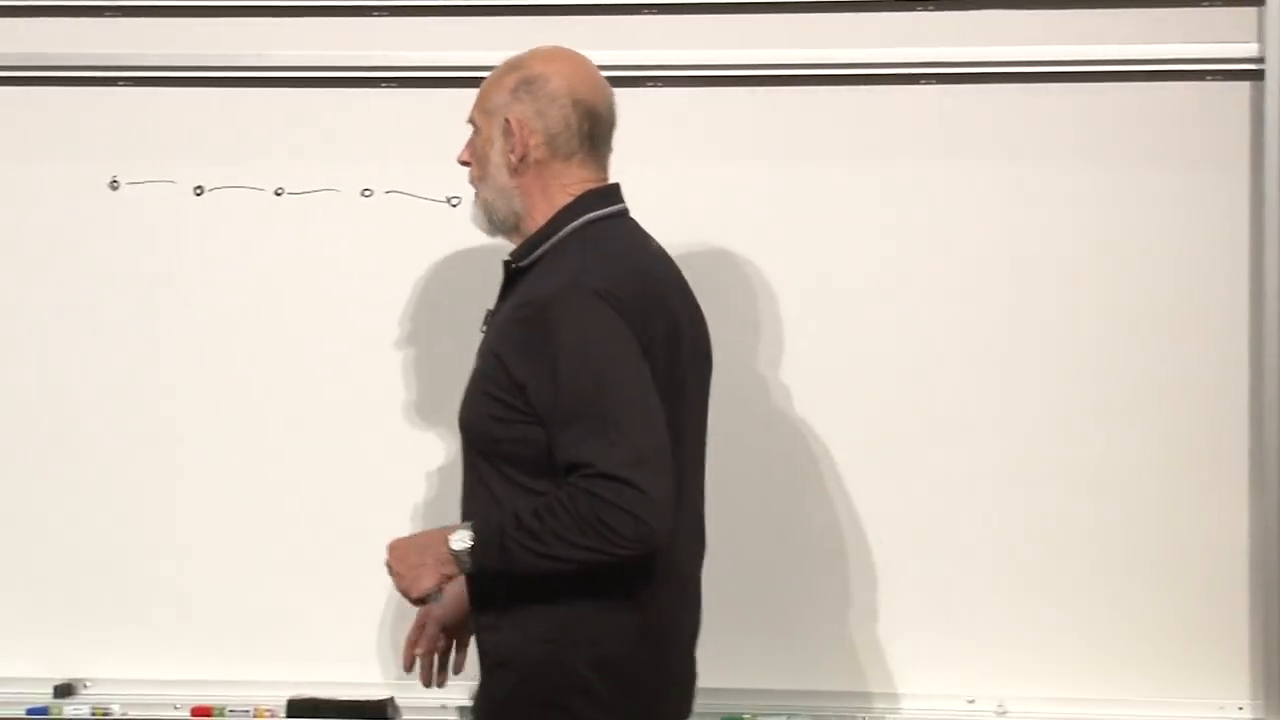
\includegraphics[width=0.92\textwidth]{lecture_04_figure_14.png}
\caption{共通の加速度が剛性を保つかどうかを調べるために用いられる隣接観測者の列。}
\end{figure}

離れた観測者が1つの慣性系に従って同一の加速度プログラムに従うなら、変化する瞬間静止系におけるそれらの間の距離は固定されたままでない。それらを結ぶ弦は伸び、最終的には切れる。これはベル宇宙船思考実験によって示されるのと同じ運動学的張力である。さらに、一定のニュートン的座標加速度は無限に続くことはできない。最終的には光より速い速度を予測することになる。

したがって、相対論的に剛体な加速系は各位置で異なる固有加速度を用いなければならない。いわゆる事象の地平面に近い観測者ほどより強く加速し、遠い観測者ほどより緩やかに加速する。そうすれば、それらの固有間隔は瞬間共動系において一定に保たれうる。これが1次元空間におけるボルン剛体加速である。

\section{ウォーミングアップとしてのユークリッド極座標}

正しい構成は、通常の円から始めると最も見やすい。ユークリッド平面において、
\begin{equation}
x=r\cos\theta,
\qquad
y=r\sin\theta,
\end{equation}
したがって
\begin{equation}
x^2+y^2=r^2,
\qquad
\cos^2\theta+\sin^2\theta=1.
\end{equation}
複素指数形式は
\begin{equation}
\cos\theta=\frac{e^{i\theta}+e^{-i\theta}}{2},
\qquad
\sin\theta=\frac{e^{i\theta}-e^{-i\theta}}{2i}.
\label{eq:l4-euler-trig}
\end{equation}
正弦公式の分母にある \(i\) の因子は、板書での議論の間に指摘され、復元される。

\begin{figure}[htbp]
\centering
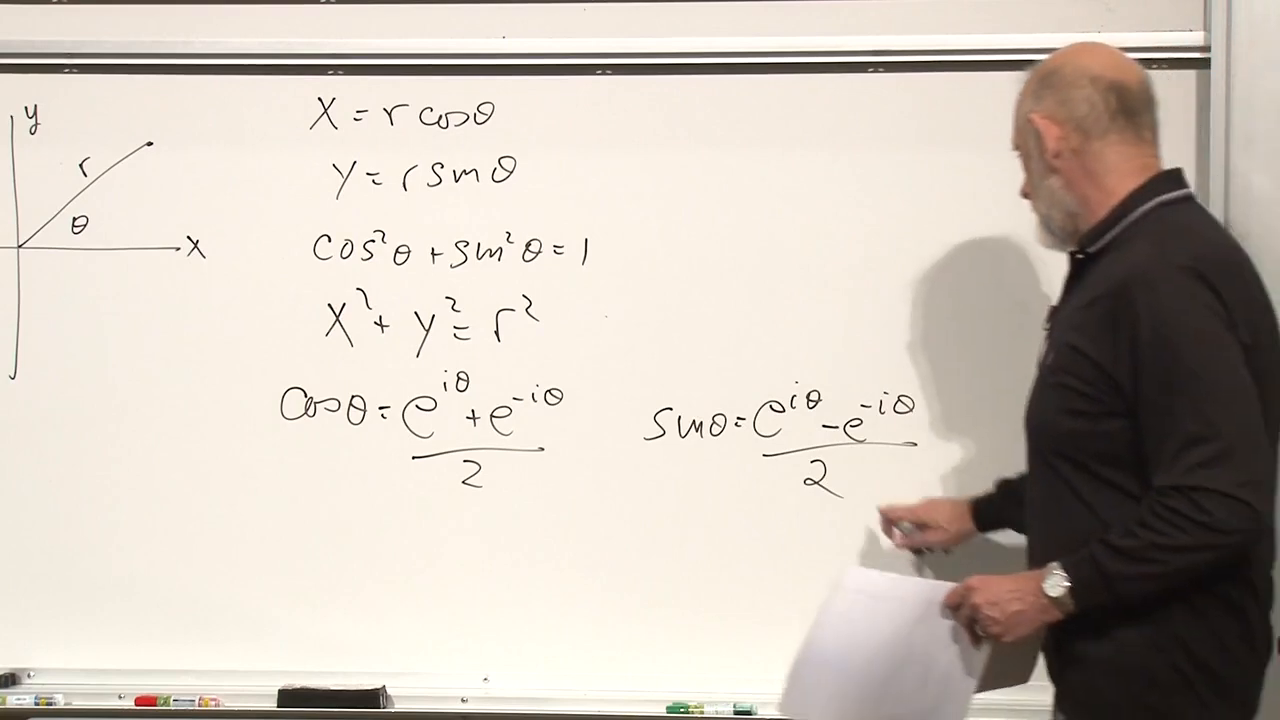
\includegraphics[width=0.94\textwidth]{lecture_04_figure_15.png}
\caption{円、ユークリッド極座標、およびそれらの指数三角関数形式。}
\end{figure}

\(r\) の固定値は円である。一定の角速度での運動は、大きさが一定の向心加速度を持ち、常に内向きである。双曲線は時空において対応する役割を果たす。

\section{ミンコフスキー時空における双曲座標}

三角関数をその双曲関数に置き換える。
\begin{equation}
\cosh\omega=\frac{e^\omega+e^{-\omega}}{2},
\qquad
\sinh\omega=\frac{e^\omega-e^{-\omega}}{2},
\end{equation}
ここで
\begin{equation}
\cosh^2\omega-\sinh^2\omega=1.
\label{eq:l4-hyperbolic-identity}
\end{equation}
\(i\) の因子はない。座標 \(\omega\) は双曲角、すなわちラピディティである。通常の角と異なり、周期的ではなく、\(-\infty\) から \(+\infty\) まで変化する。

\begin{figure}[htbp]
\centering
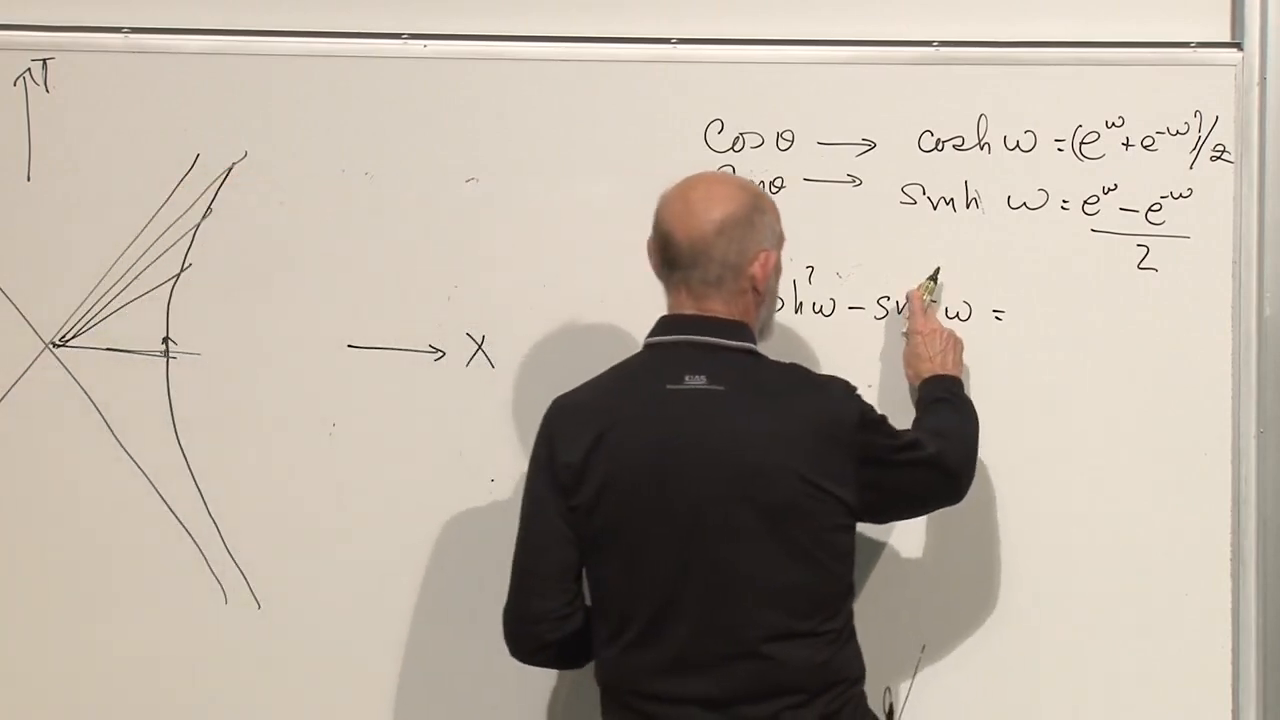
\includegraphics[width=0.94\textwidth]{lecture_04_figure_16.png}
\caption{時空の構成において円関数が双曲関数に置き換えられる。}
\end{figure}

右リンドラー楔において新しい座標を定義する。
\begin{equation}
x=r\cosh\omega,
\qquad
t=r\sinh\omega,
\qquad
r>0.
\label{eq:l4-rindler-transform}
\end{equation}
すると
\begin{equation}
x^2-t^2=r^2.
\label{eq:l4-rindler-hyperbola}
\end{equation}
\(r\) を固定して \(\omega\) を変化させると双曲線を描く。\(r\) を増やすと、その族を空間的方向に横切って移動し、\(\omega\) を増やすと、1つの双曲線に沿って時間的方向に前方へ移動する。

\begin{figure}[htbp]
\centering
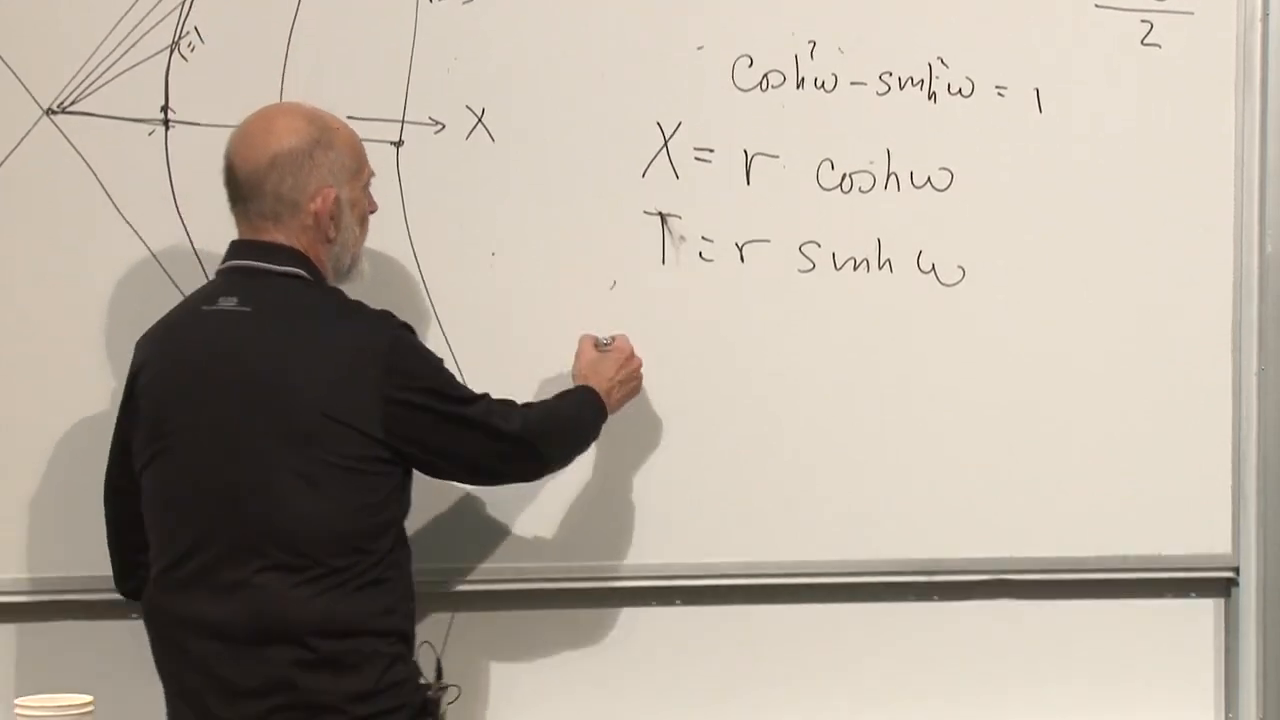
\includegraphics[width=0.94\textwidth]{lecture_04_figure_17.png}
\caption{座標変換 \(x=r\cosh\omega\)、\(t=r\sinh\omega\)、およびその不変双曲線。}
\end{figure}

\begin{figure}[htbp]
\centering
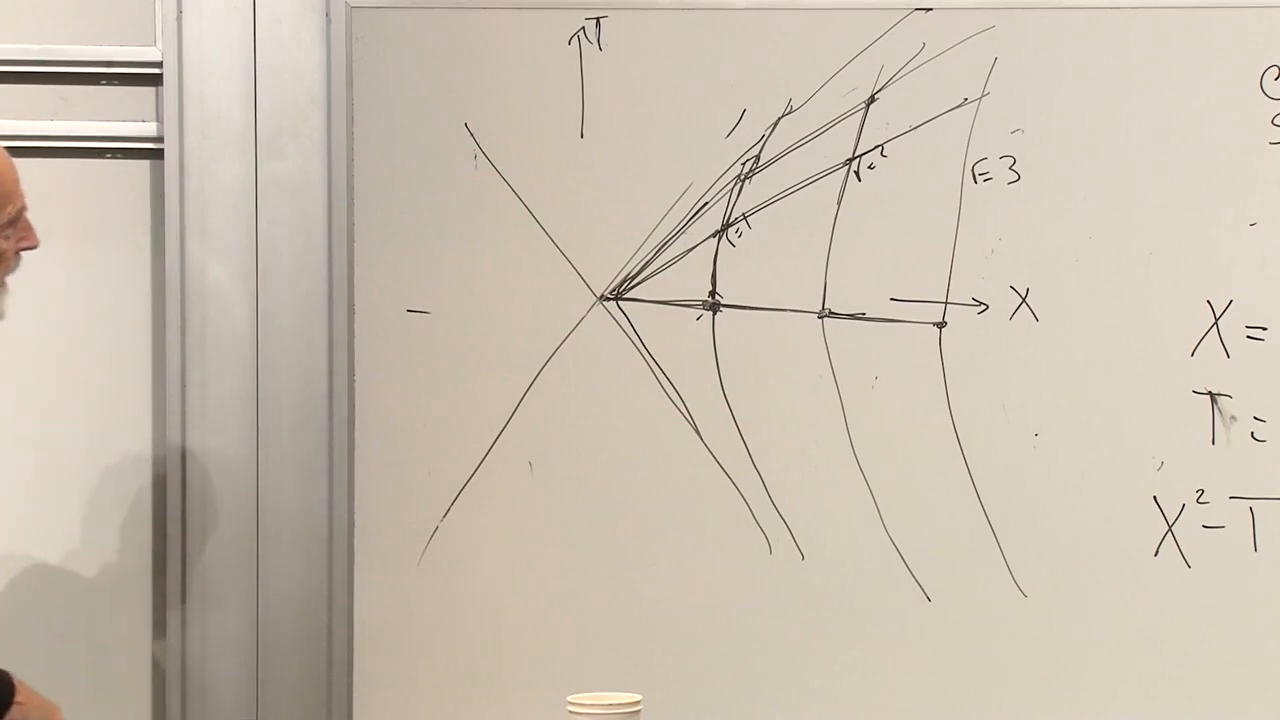
\includegraphics[width=0.94\textwidth]{lecture_04_figure_18.png}
\caption{剛体加速された族を表す固定 \(r\) の双曲線の合同族。}
\end{figure}

\subsection{加速座標における計量}

\eqref{eq:l4-rindler-transform} を微分する。
\begin{align}
dx&=\cosh\omega\,dr+r\sinh\omega\,d\omega,\\
dt&=\sinh\omega\,dr+r\cosh\omega\,d\omega.
\end{align}
\eqref{eq:l4-hyperbolic-identity} を用いると、交差項は相殺される。
\begin{align}
d\tau^2
&=dt^2-dx^2\\
&=r^2\,d\omega^2-dr^2.
\label{eq:l4-rindler-metric}
\end{align}
横方向は、復元すると、ここで用いた固有時規約に単に \(-dy^2-dz^2\) を加える。

これは依然として平坦な時空である。座標に依存する係数\(r^2\)は、ユークリッド極座標において\(d\theta^2\)に掛かる\(r^2\)以上に曲率の証拠にはならない。

\subsection{双曲線上に沿った固有加速度}

固定された世界線\(r=R\)に対して、式\eqref{eq:l4-rindler-metric}は次を与える：
\begin{equation}
d\tau=R\,d\omega.
\end{equation}
その四元速度は
\begin{equation}
U^\mu
=
\frac{d(t,x)}{d\tau}
=
(\cosh\omega,\sinh\omega),
\end{equation}
であり、その四元加速度は
\begin{equation}
A^\mu
=
\frac{dU^\mu}{d\tau}
=
\frac{1}{R}(\sinh\omega,\cosh\omega).
\end{equation}
である。不変的な大きさは一定である：
\begin{equation}
a=\sqrt{A^\mu A_\mu}=\frac{1}{R}
\qquad (c=1).
\label{eq:l4-proper-acceleration}
\end{equation}

\begin{figure}[htbp]
\centering
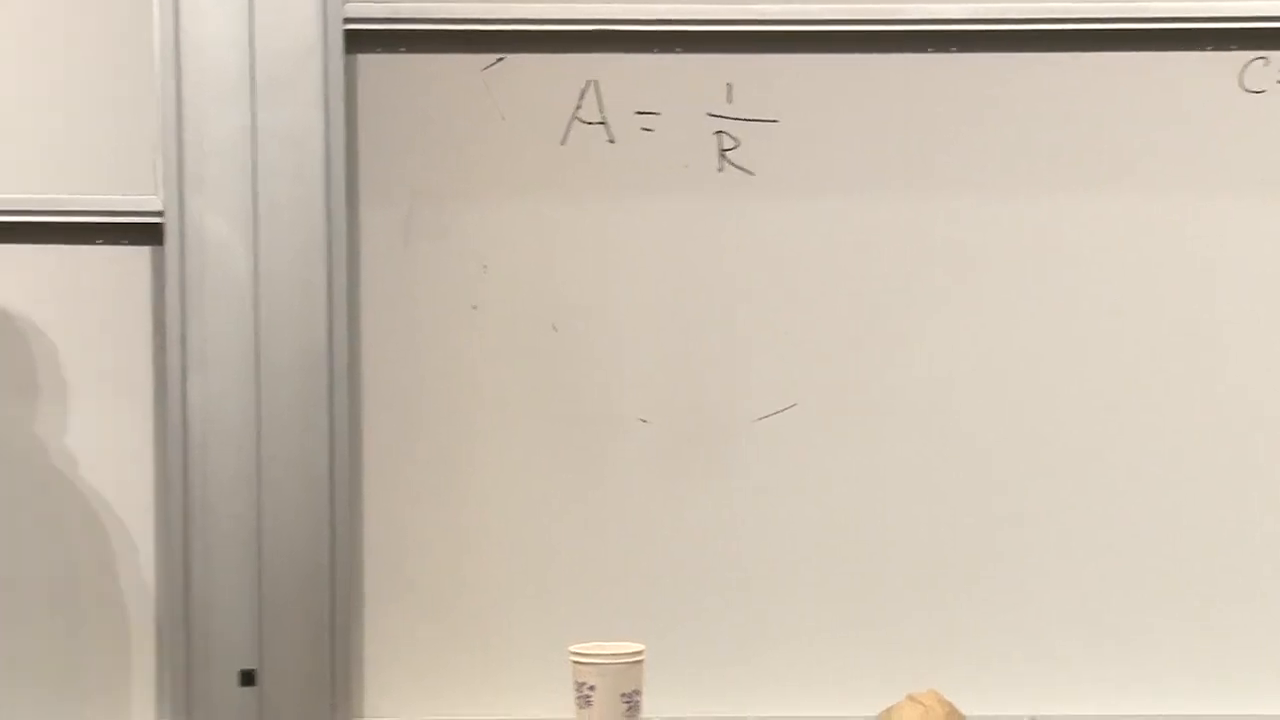
\includegraphics[width=0.90\textwidth]{lecture_04_figure_19.png}
\caption{固定された加速世界線に対する逆半径則\(a=1/R\)。}
\end{figure}

単位を復元すると、
\begin{equation}
\boxed{a=\frac{c^2}{R}.}
\label{eq:l4-proper-acceleration-units}
\end{equation}

\begin{figure}[htbp]
\centering
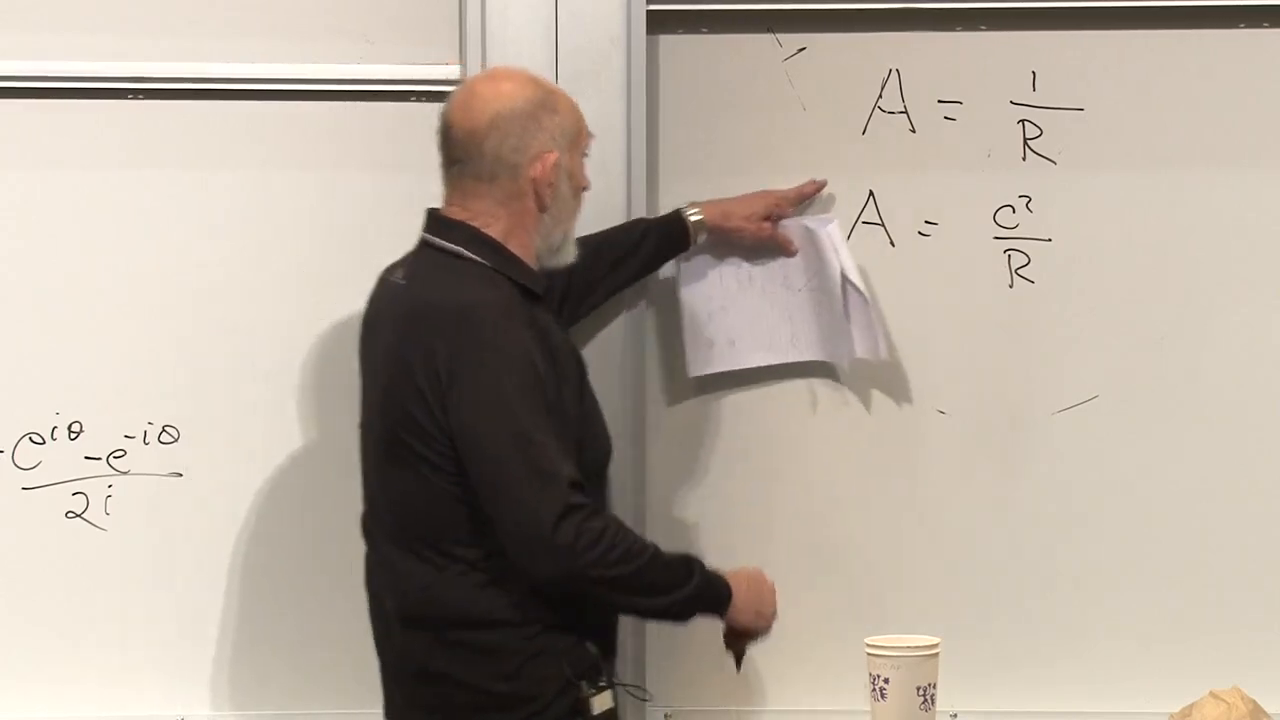
\includegraphics[width=0.90\textwidth]{lecture_04_figure_20.png}
\caption{単位を復元すると\(1/R\)が\(c^2/R\)に変換される。}
\end{figure}

切片\(R\)が小さいほど、世界線はより鋭く曲がり、その観測者が感じる固有加速度は大きくなる。より遠い双曲線は曲がりが少なく、必要な加速度も小さい。各観測者は時間に対して一定の加速度を持つが、異なる観測者は異なる加速度を持つ。その変動こそが、彼らの相互の固有距離を保つのである。

\subsection{加速座標に関する問い}

\paragraph{\(R\)は\(x\)切片か？}
はい。\(\omega=0\)において、式\eqref{eq:l4-rindler-transform}は\(t=0\)および\(x=R\)を与える。切片は\eqref{eq:l4-proper-acceleration-units}を通じて固有加速度を定める。

\paragraph{この構成は選ばれた原点に依存するか？}
座標は依存する。原点を平行移動すると、漸近線がずれた別の双曲線族が生じる。いかなる不変的な物理もその選択に依存しない。我々は意図的に一つの加速座標系を選び、その中で記述したときに慣性運動がどのように見えるかを問うているのである。

\paragraph{固有加速度とは何か？}
それは観測者が携帯する加速度計によって測定される加速度である。共変的には、
\begin{equation}
A^\mu=\frac{dU^\mu}{d\tau},
\qquad
U^\mu=\frac{dx^\mu}{d\tau}.
\end{equation}
その大きさは観測者が実際に感じる押しであり、遠方の枠が割り当てる座標加速度\(d^2x/dt^2\)ではない。

\section{極座標および双曲座標における平坦計量}

地球近傍に局所化する前に、ユークリッド計量とローレンツ計量を並べて置くと有用である。平面において、
\begin{equation}
ds^2=dr^2+r^2d\theta^2,
\qquad
g_{ab}
=
\begin{pmatrix}
1&0\\
0&r^2
\end{pmatrix}.
\label{eq:l4-polar-metric}
\end{equation}
聴衆からの提案が球面因子を簡単に導入するが、これは単なる平面であり、球面ではない。\(r^2\)項は、固定された角度間隔がより大きな半径においてより長い弧にわたるという事実を記録している。

\begin{figure}[htbp]
\centering
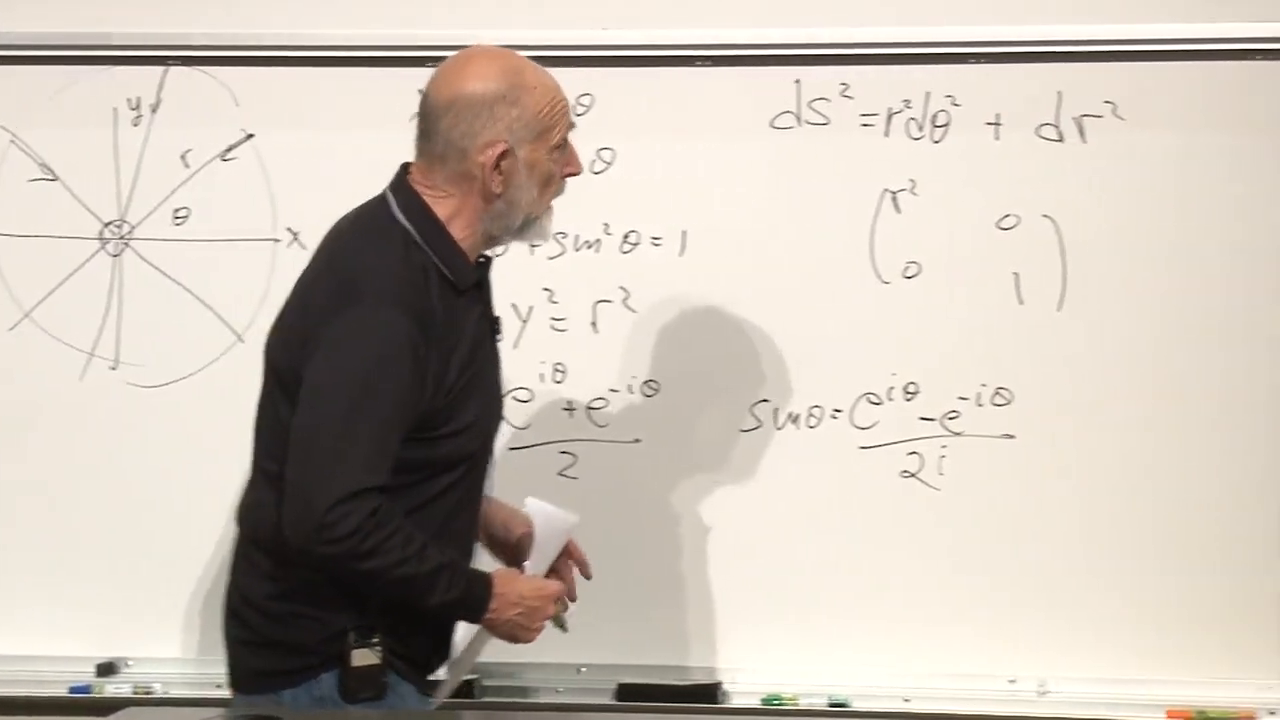
\includegraphics[width=0.94\textwidth]{lecture_04_figure_21.png}
\caption{ユークリッド極座標計量：平坦な平面における位置依存成分。}
\end{figure}

ミンコフスキー版の類似は
\begin{equation}
d\tau^2=r^2d\omega^2-dr^2.
\end{equation}
である。両方の計量は位置依存の成分を持つが、両方の幾何学は平坦である。座標の曲率と幾何学的曲率は同じものではない。

\section{地球の加速度近傍への局所化}

固有加速度が地球の値\(g\)である一つの参照双曲線を選ぶ：
\begin{equation}
g=\frac{c^2}{R},
\qquad
R=\frac{c^2}{g}.
\label{eq:l4-earth-radius}
\end{equation}

\begin{figure}[htbp]
\centering
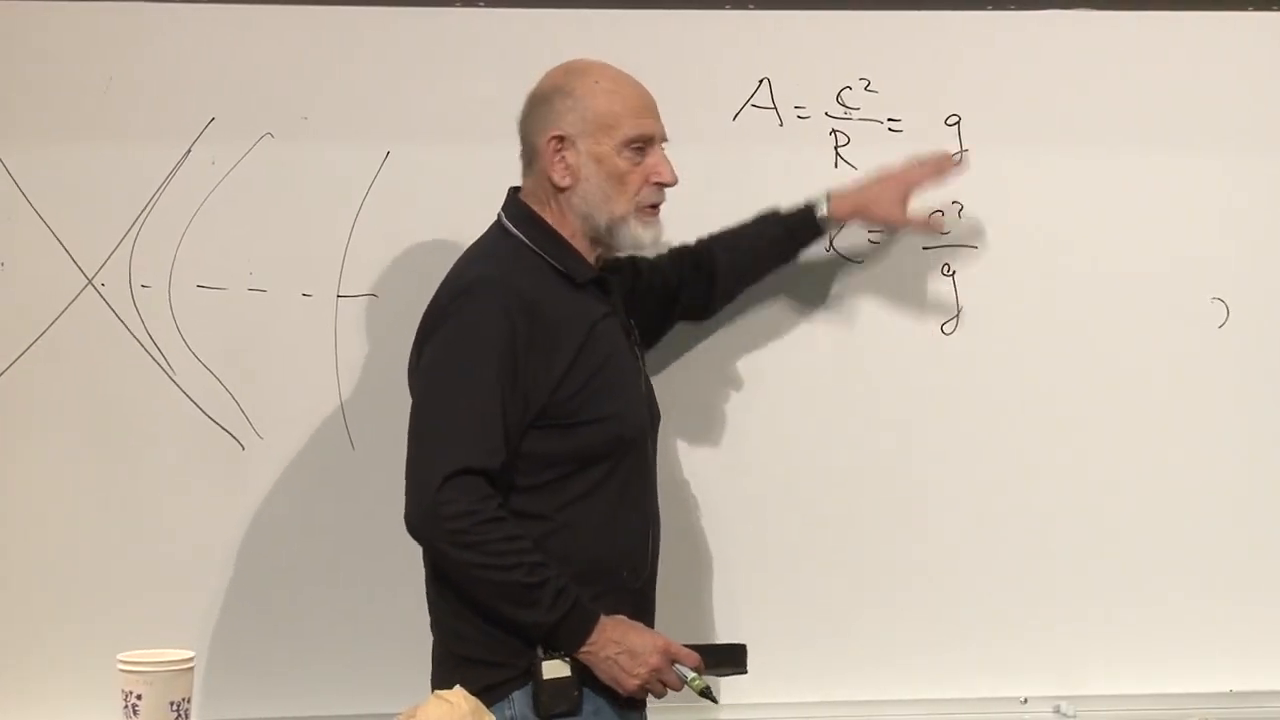
\includegraphics[width=0.94\textwidth]{lecture_04_figure_22.png}
\caption{\(c^2/R=g\)によって参照双曲線を選択する。}
\end{figure}

数値的には、
\begin{equation}
R
\simeq
\frac{(3.0\times10^8\ {\rm m\,s^{-1}})^2}
{9.8\ {\rm m\,s^{-2}}}
\simeq
9.2\times10^{15}\ {\rm m}.
\end{equation}
講義ではこれを\(10^{16}\)メートルに丸める。地球の\(g\)の場は相対論的スケールでは控えめであるため、対応するリンドラー半径は膨大である。

ここで、その参照観測者の小さな近傍のみを調べる。局所的な高さ\(y\)を次によって導入する：
\begin{equation}
r=R+y,
\qquad
dr=dy,
\qquad
|y|\ll R.
\label{eq:l4-local-height}
\end{equation}
等式\(dr=dy\)は議論中に明示的に指摘されるため、空間項は\(-dy^2\)と書かなければならない。

\eqref{eq:l4-rindler-metric}への代入は次を与える：
\begin{align}
d\tau^2
&=(R+y)^2d\omega^2-dy^2\\
&=(R^2+2Ry+y^2)d\omega^2-dy^2\\
&=
\left(
1+\frac{2y}{R}+\frac{y^2}{R^2}
\right)
R^2d\omega^2-dy^2.
\label{eq:l4-local-expand}
\end{align}

\begin{figure}[htbp]
\centering
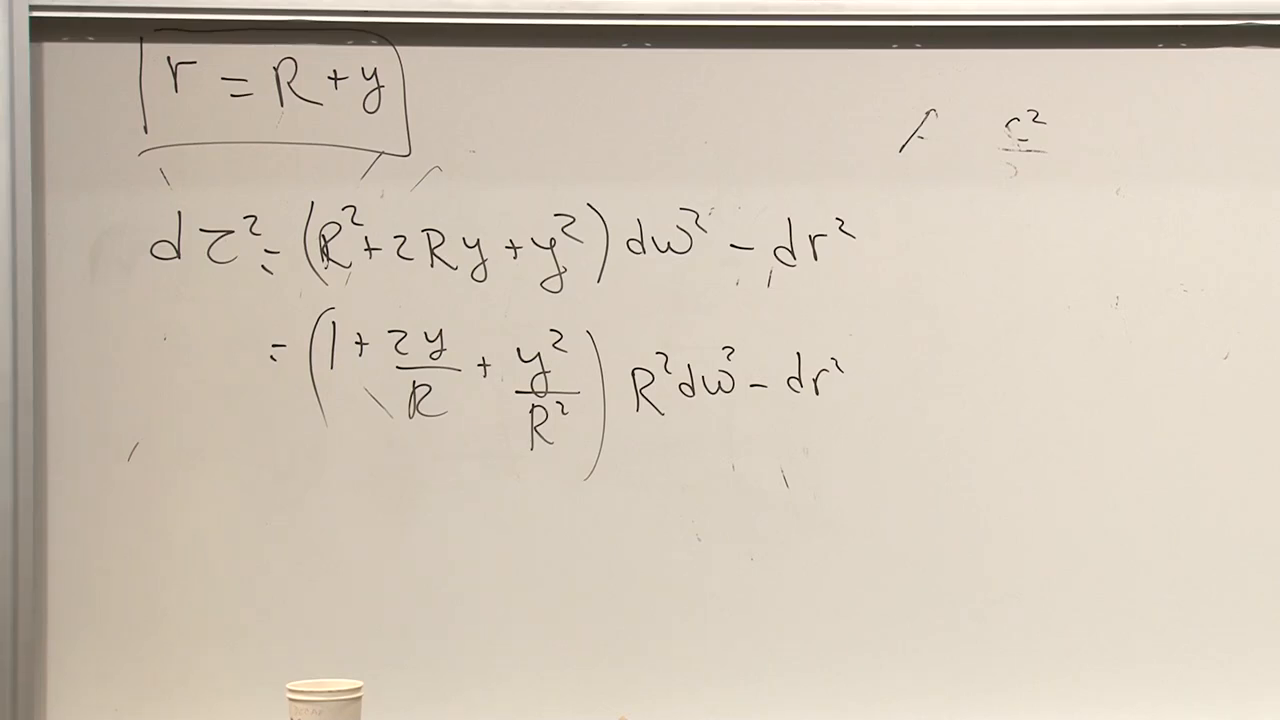
\includegraphics[width=0.94\textwidth]{lecture_04_figure_23.png}
\caption{\(r=R+y\)の周りで加速計量を展開する。}
\end{figure}

局所時間座標を定義する：
\begin{equation}
t=R\omega.
\label{eq:l4-local-time}
\end{equation}
すると
\begin{equation}
d\tau^2
=
\left(
1+\frac{2y}{R}+\frac{y^2}{R^2}
\right)dt^2-dy^2.
\label{eq:l4-local-exact}
\end{equation}

\begin{figure}[htbp]
\centering
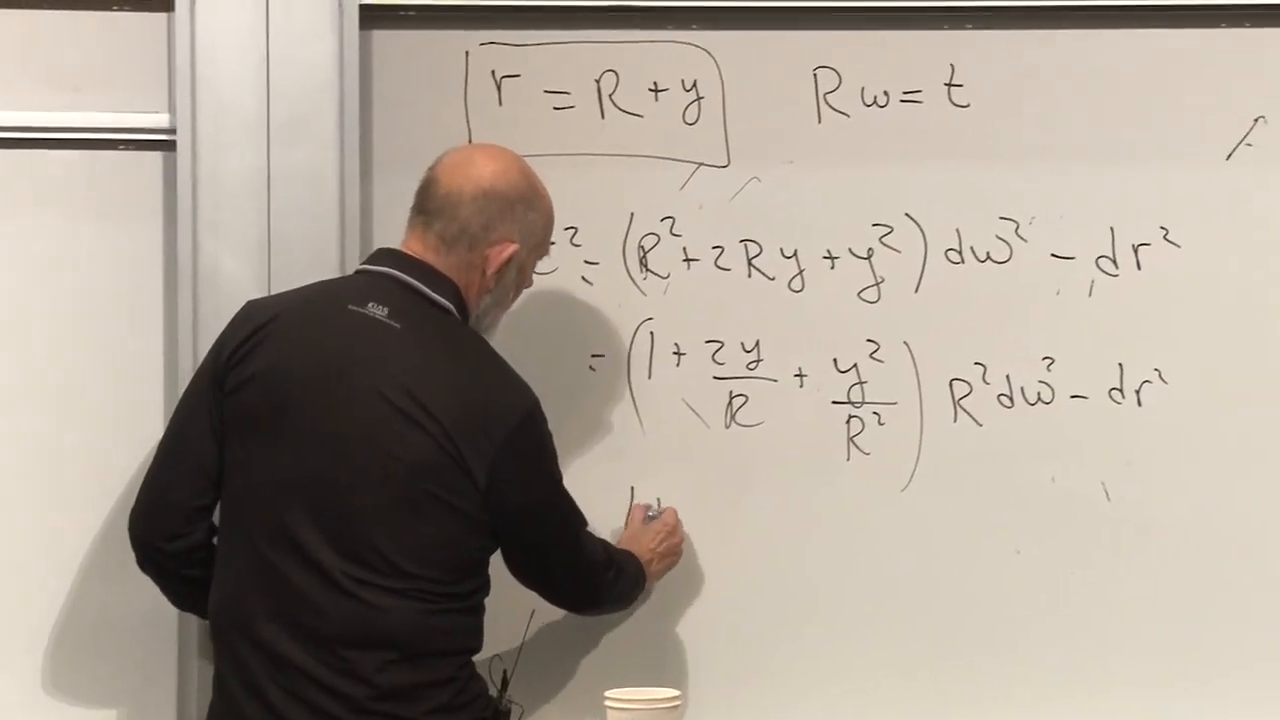
\includegraphics[width=0.94\textwidth]{lecture_04_figure_24.png}
\caption{参照双曲線の周りでの展開後に\(t=R\omega\)を導入する。}
\end{figure}

数十キロメートルの垂直方向の移動でさえ\(R\)に比べて微小である。講義では比較を鮮明にするために約二十四マイルの落下を用いる：そのような距離は\(10^{16}\)メートルの隣では依然として無視できる。したがって\(y^2/R^2\)は\(y/R\)よりはるかに小さく、二次項は落としてよい：
\begin{equation}
d\tau^2
\simeq
\left(1+\frac{2y}{R}\right)dt^2-dy^2.
\label{eq:l4-local-linear}
\end{equation}

\begin{figure}[htbp]
\centering
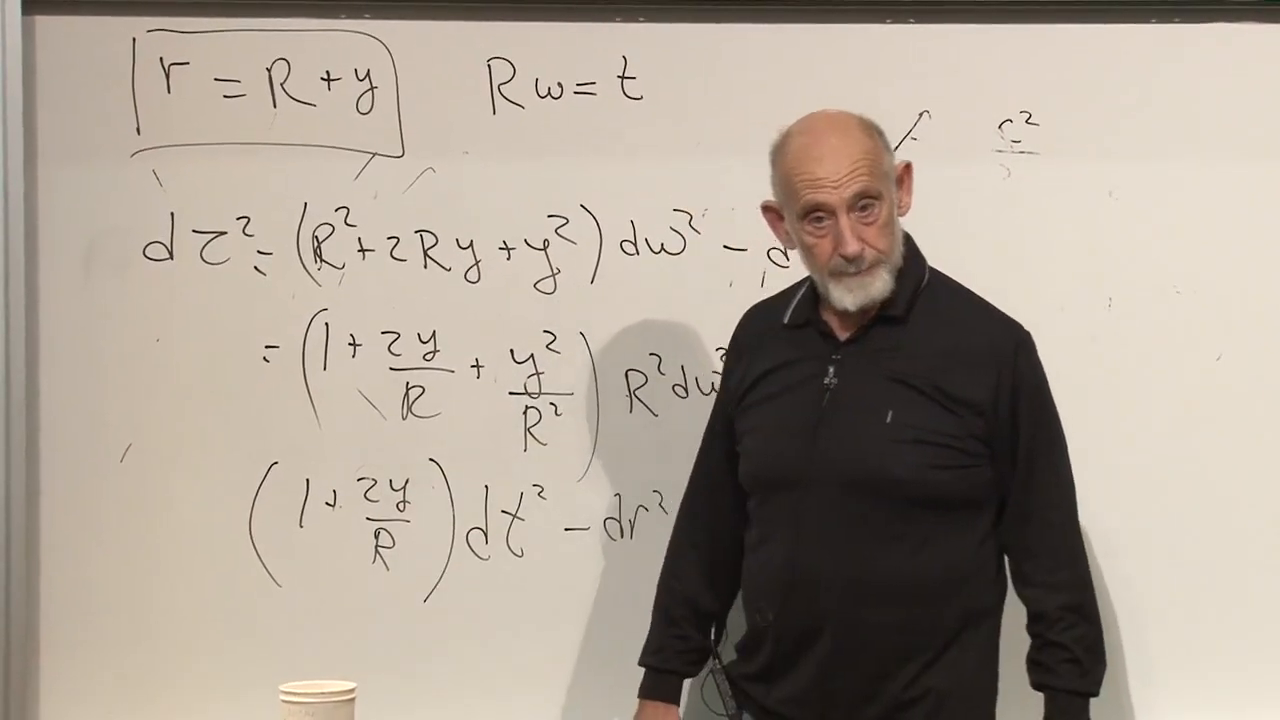
\includegraphics[width=0.94\textwidth]{lecture_04_figure_25.png}
\caption{弱場切断前の展開計量と局所時間の代入。}
\end{figure}

\(c=1\)とする単位では、式\eqref{eq:l4-earth-radius}は\(1/R=g\)を与え、したがって
\begin{equation}
\boxed{
d\tau^2\simeq(1+2gy)\,dt^2-dy^2.
}
\label{eq:l4-uniform-metric}
\end{equation}

\begin{figure}[htbp]
\centering
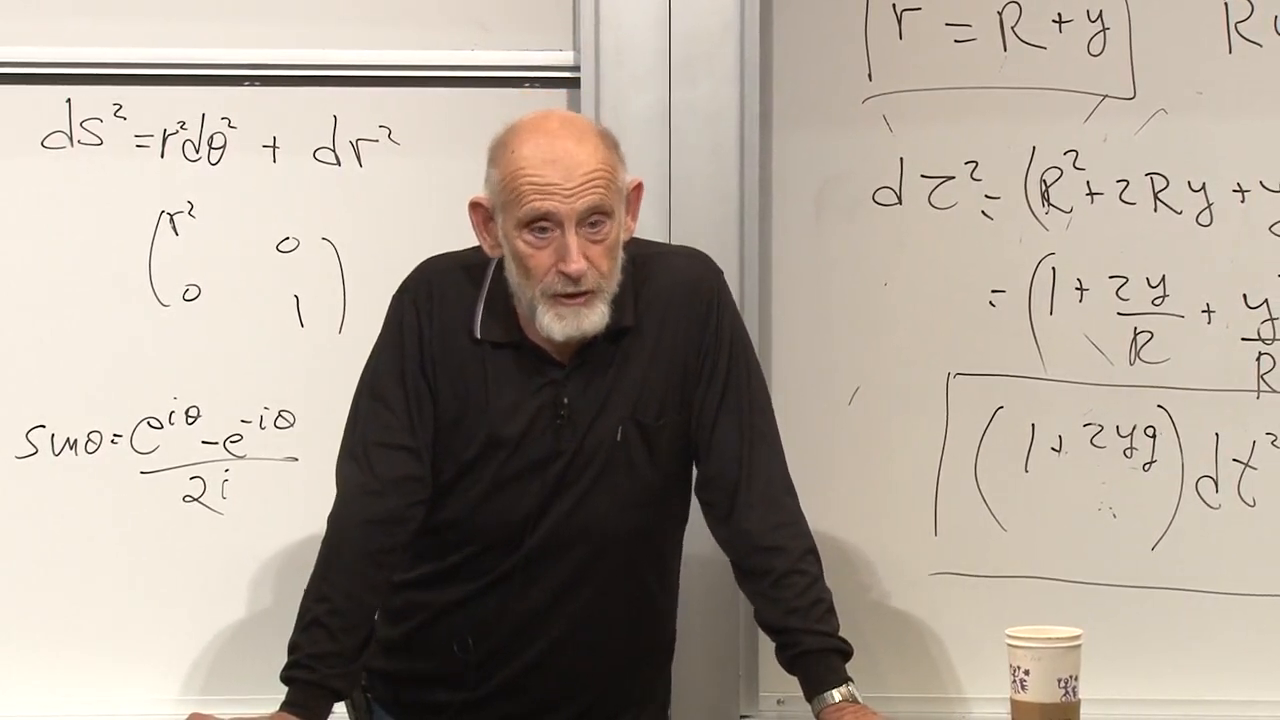
\includegraphics[width=0.94\textwidth]{lecture_04_figure_26.png}
\caption{一様に加速するエレベーターに対する完成した局所計量。}
\end{figure}

量
\begin{equation}
\Phi(y)=gy
\end{equation}
は一様場における単位質量あたりのニュートン重力ポテンシャルである。したがって
\begin{equation}
d\tau^2\simeq(1+2\Phi)\,dt^2-dy^2
\qquad (c=1).
\label{eq:l4-weak-potential-propertime}
\end{equation}
講義の規約\(d\tau^2=-g_{\mu\nu}dx^\mu dx^\nu\)では、これは次を意味する：
\begin{equation}
g_{tt}=-(1+2\Phi).
\label{eq:l4-gtt-potential}
\end{equation}
従来の単位では、無次元の補正は\(2\Phi/c^2\)である。

何も時空を曲げていない。式\eqref{eq:l4-uniform-metric}は平坦なリンドラー計量の局所展開である。その見かけの重力は、加速されたエレベーターの内部で見られる慣性力である。

\section{測地線方程式がニュートンの法則になる}

\(gy\)をポテンシャルと同一視することは、これまで示唆的であった。決定的な検証は動力学的である。計量\eqref{eq:l4-uniform-metric}中の自由粒子は\(d^2y/dt^2=-g\)で下方へ加速するか？

固有時間でパラメータ付けられた時間的世界的線に対して、
\begin{equation}
\frac{d^2x^\nu}{d\tau^2}
+\Gamma^\nu{}_{\mu\rho}
\frac{dx^\mu}{d\tau}
\frac{dx^\rho}{d\tau}
=0.
\label{eq:l4-spacetime-geodesic}
\end{equation}
鉛直成分は
\begin{equation}
\frac{d^2y}{d\tau^2}
=
-\Gamma^y{}_{\mu\rho}
\frac{dx^\mu}{d\tau}
\frac{dx^\rho}{d\tau}.
\label{eq:l4-y-geodesic}
\end{equation}

\begin{figure}[htbp]
\centering
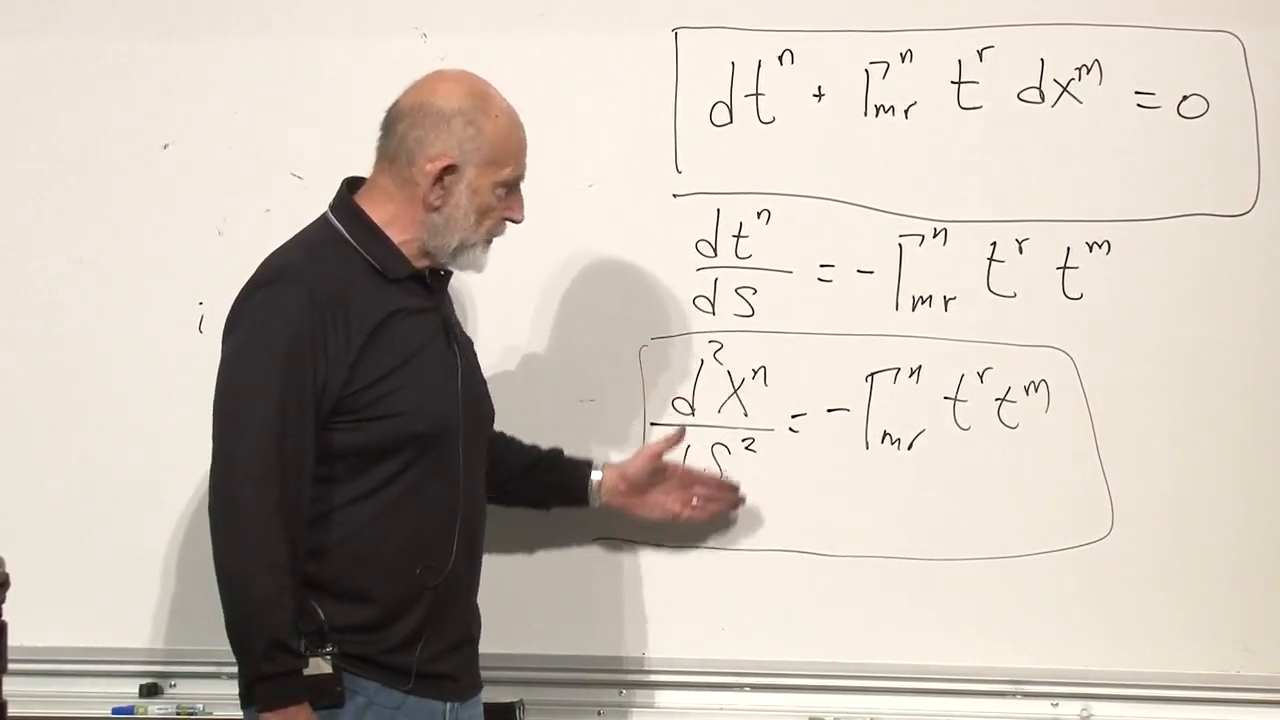
\includegraphics[width=0.94\textwidth]{lecture_04_figure_27.png}
\caption{輸送方程式とその二階の測地線形。鉛直運動に適用する準備が整った。}
\end{figure}

\subsection{低速運動近似}

弱い静的場の中をゆっくり運動する粒子に対して、
\begin{equation}
\frac{dt}{d\tau}\simeq1,
\qquad
\left|\frac{dy}{d\tau}\right|\ll1.
\end{equation}
したがって四元速度の時間成分はオーダー1であり、空間成分はそれに比べて小さい。\eqref{eq:l4-y-geodesic}中の積のうち、支配的なものは\(\mu=\rho=t\)を持つ：
\begin{equation}
\frac{d^2y}{d\tau^2}
\simeq
-\Gamma^y{}_{tt}
\left(\frac{dt}{d\tau}\right)^2
\simeq
-\Gamma^y{}_{tt}.
\label{eq:l4-slow-geodesic}
\end{equation}

\begin{figure}[htbp]
\centering
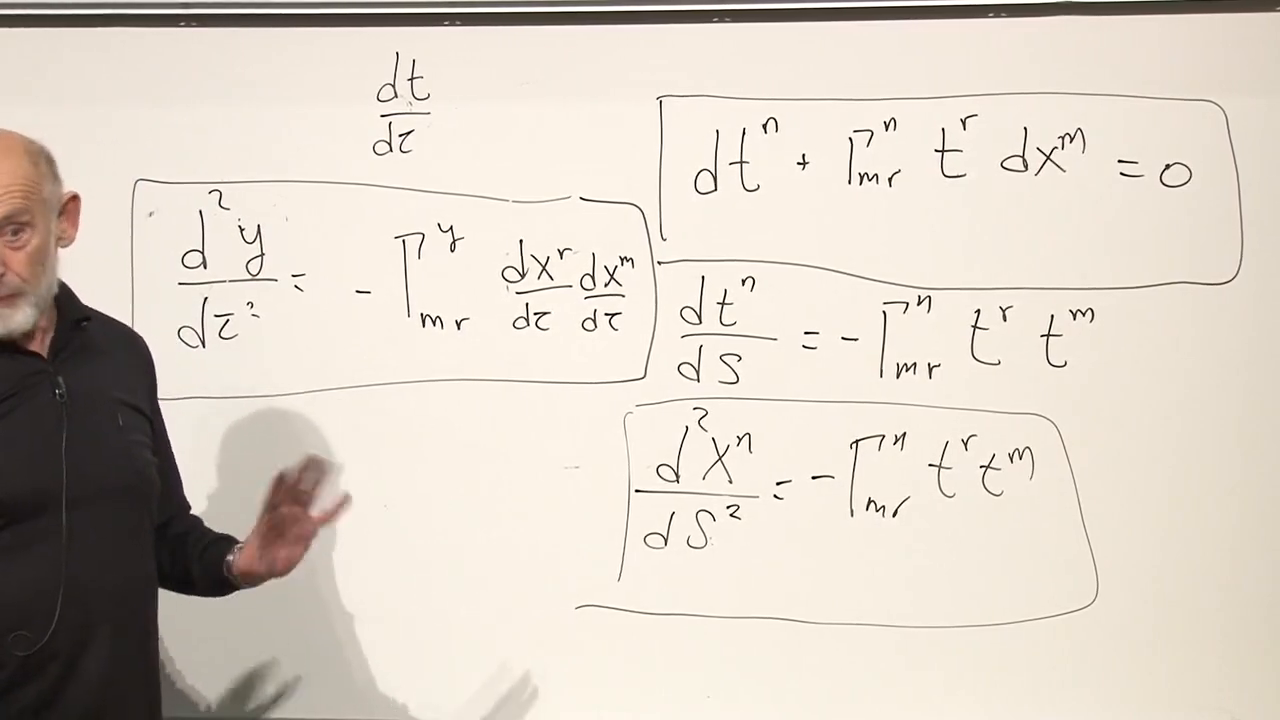
\includegraphics[width=0.94\textwidth]{lecture_04_figure_28.png}
\caption{時空の測地線方程式をゆっくり運動する\(y\)成分に特殊化する。}
\end{figure}

次に、必要な接続係数を一つ計算する。計量は対角的で\(t\)に依存しないので、
\begin{align}
\Gamma^y{}_{tt}
&=
\frac{1}{2}g^{yy}
\left(
\partial_tg_{yt}
+\partial_tg_{ty}
-\partial_yg_{tt}
\right)\\
&=
-\frac{1}{2}\partial_yg_{tt},
\label{eq:l4-gamma-ytt}
\end{align}
なぜなら、講義のmostly-plusテンソル規約では\(g^{yy}=1\)だからである。

\begin{figure}[htbp]
\centering
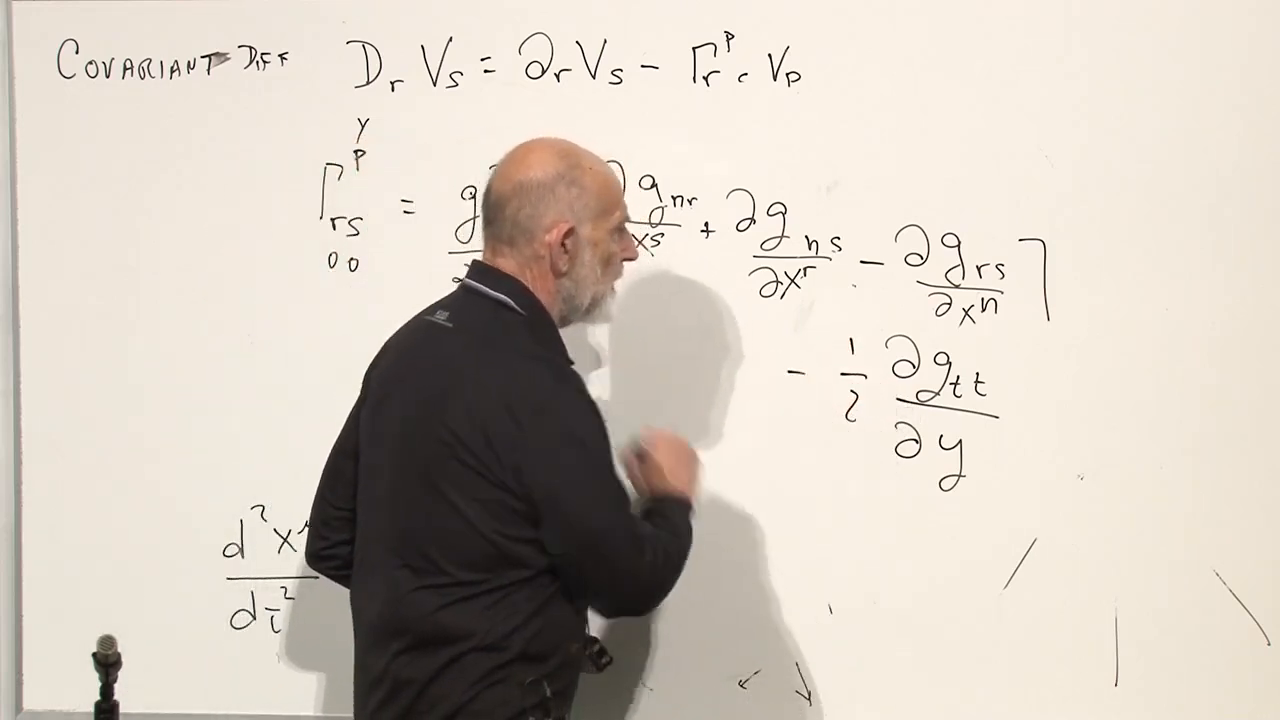
\includegraphics[width=0.94\textwidth]{lecture_04_figure_29.png}
\caption{クリストッフェルの公式を\(y,t,t\)成分に還元した。}
\end{figure}

\eqref{eq:l4-slow-geodesic}と\eqref{eq:l4-gamma-ytt}を組み合わせると、
\begin{equation}
\frac{d^2y}{d\tau^2}
\simeq
\frac{1}{2}\partial_yg_{tt}.
\label{eq:l4-accel-gtt}
\end{equation}
\eqref{eq:l4-gtt-potential}から、
\begin{equation}
\partial_yg_{tt}
=
-2\partial_y\Phi
=
-2g.
\end{equation}
したがって
\begin{equation}
\boxed{
\frac{d^2y}{d\tau^2}=-g.
}
\label{eq:l4-newton-result}
\end{equation}
同じ低速運動近似で\(t\simeq\tau\)なので、これはまた
\begin{equation}
\frac{d^2y}{dt^2}=-g.
\end{equation}

\begin{figure}[htbp]
\centering
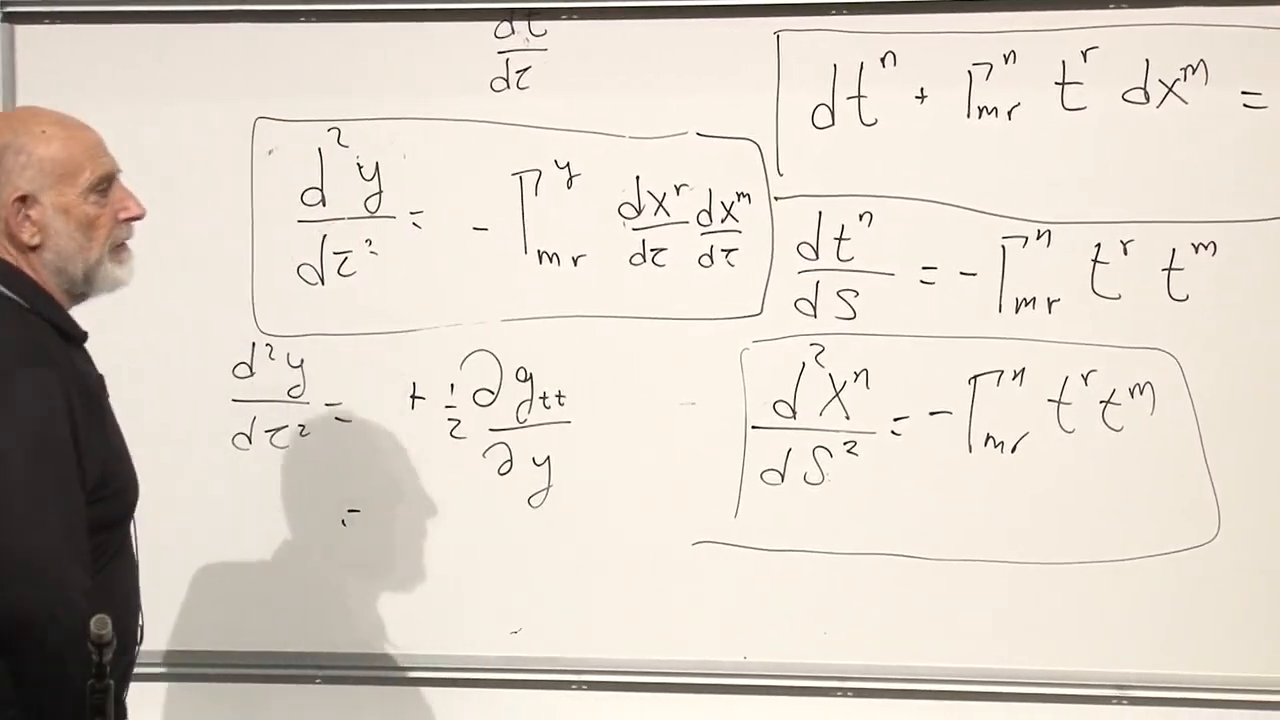
\includegraphics[width=0.94\textwidth]{lecture_04_figure_30.png}
\caption{完成した符号の連鎖：\(g_{tt}\)の\(y\)微分が加速度\(-g\)を生じる。}
\end{figure}

より一般に、ニュートン領域では、
\begin{equation}
\boxed{
\begin{aligned}
g_{tt}&=-(1+2\Phi),\\
\frac{d^2x^i}{dt^2}&=-\partial_i\Phi
\end{aligned}
}
\qquad(c=1).
\label{eq:l4-newton-general}
\end{equation}
単位を復元すると、計量の補正は\(2\Phi/c^2\)であり、加速度は\(-\boldsymbol{\nabla}\Phi\)のままである。

この計算は、なぜ別個の重力場ではなく計量が中心的な対象であるかを説明する。自由粒子は単に時空の測地線に従う。加速された実験室に適合した座標では、その測地線は通常重力に帰される座標曲率を持つ。

\subsection{選ばれたリンドラー原点に関する問い}

基準双曲線をずらして、その漸近線と切片が別の場所に現れるようにすることはできたか？ できる。適切に平行移動された原点のそれぞれに対して、一様加速座標系が存在する。エレベーターの描像では、これらの選択は、ある瞬間に床が異なる位置を占めるエレベーターを選ぶことに相当する。

局所的な結果は特権的な原点に依存しない。加速度\(g\)を持つ基準観測者が選ばれれば、\(y\)はその観測者に対する高さを測り、近傍の計量は\eqref{eq:l4-uniform-metric}の形をとる。任意の座標選択は、床をどこで記述するかを決めるが、不変な曲率を生み出すわけではない。

\section{なぜクリストッフェル記号はテンソルであってはならないのか}

講義後の議論は、復習中に最初に現れた点に戻る。元の慣性座標では、
\begin{equation}
g_{\mu\nu}=\eta_{\mu\nu},
\qquad
\partial_\rho\eta_{\mu\nu}=0,
\qquad
\Gamma^\mu{}_{\nu\rho}=0.
\end{equation}
自由粒子は直線上を運動し、重力は存在しない。

加速座標では、同じ平坦な時空が位置に依存する計量成分を持つ。そのクリストッフェル記号は消えず、同じ慣性軌道が曲がって見える。粒子はエレベーターの床に向かって落ちるように見える。

もし\(\Gamma^\mu{}_{\nu\rho}\)がテンソルであれば、これは不可能であろう。ある枠で消えるテンソルはすべての枠で消える。それに対して接続は座標変換の下で非斉次項を獲得するので、慣性枠ではゼロであり、加速枠では非ゼロでありうる。これはまさに等価原理が要求するものである：
\begin{equation}
\text{accelerated frame}
\quad\longleftrightarrow\quad
\text{local gravity}.
\end{equation}

曲率は異なる振る舞いをする。リーマンテンソルはテンソルである。もしそれが慣性枠で消えるなら、加速枠でも同様に消える：
\begin{equation}
R^\mu{}_{\nu\rho\sigma}=0.
\end{equation}
したがってクリストッフェル記号は座標に依存する重力を記述し、曲率は座標の変更では取り除けない不変な潮汐的内容を検出する。

\section{一様ポテンシャルからシュヴァルツシルトの予告へ}

加速されたエレベーターには重力を及ぼす物質も曲率もない。それにもかかわらず、弱場の関係\eqref{eq:l4-newton-general}は、実際の球対称質量の場で何を探すべきかを示唆する。質量\(M\)の外側のニュートンポテンシャルは
\begin{equation}
\Phi(r)=-\frac{GM}{r}.
\label{eq:l4-newton-potential}
\end{equation}
これを弱場の時間成分に代入すると
\begin{equation}
g_{tt}
\simeq
-\left(1-\frac{2GM}{r}\right)
\qquad(c=1).
\label{eq:l4-schwarzschild-preview}
\end{equation}
ポテンシャルの符号は板書の議論の間に修正される。引力は、\(r\)が無限大に近づくにつれて下からゼロに近づく負のポテンシャルを必要とする。

\begin{figure}[htbp]
\centering
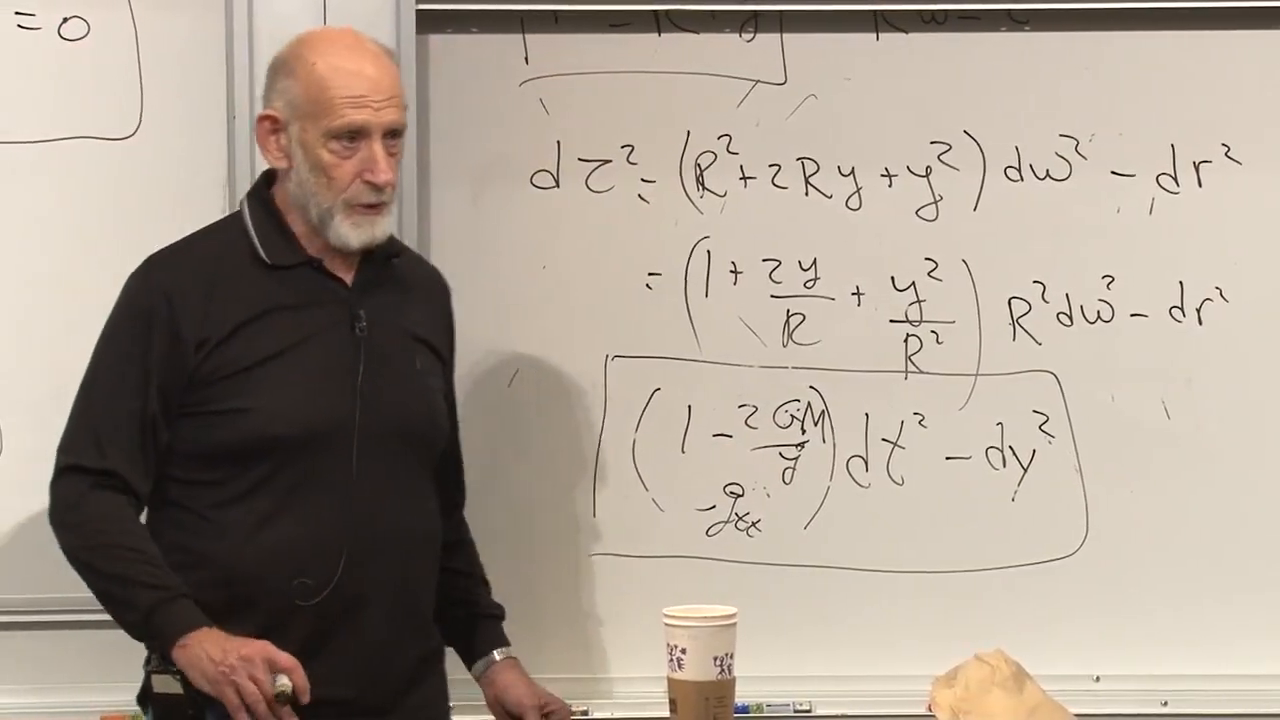
\includegraphics[width=0.94\textwidth]{lecture_04_figure_31.png}
\caption{ニュートンポテンシャルを時間-時間計量係数に代入すると、因子\(1-2GM/r\)が現れる。}
\end{figure}

この係数は
\begin{equation}
r=2GM
\qquad(c=1),
\end{equation}
で消える。あるいは単位を復元すれば、
\begin{equation}
r_s=\frac{2GM}{c^2}.
\end{equation}
である。これがシュヴァルツシルト半径である。この特定の計量係数が消えることは、事象の地平面を予兆している。

この議論は、導出ではなく予告として意図的に提示されている。弱場近似だけでは、\(r=2GM/c^2\)の近傍、すなわちまさに補正がもはや小さくない領域において、厳密なシュヴァルツシルト解を確立することはできない。完全な解はまた、非自明な動径成分を含み、アインシュタインの場の方程式を満たさなければならない。それらの方程式はまだ導入されていない。現在の推論が明らかにするのは、正しい構造上の手がかりと、質的に新しい何かが起こらなければならないスケールである。

\section{教室での質問と訂正}

\subsection{双曲角は通常の角のように振る舞うか。}

いいえ。両者とも一定半径の曲線族に沿った運動をパラメータ付けするが、\(\theta\)は周期的であるのに対し、ラピディティ\(\omega\)は実数直線全体を動く。角という語は、回転とローレンツブーストの間の代数的な類似を指しており、\(0\)と\(2\pi\)の間に制限された量を指すのではない。

\subsection{なぜ控えめな加速度に巨大なRが必要なのか。}

関係\(a=c^2/R\)には、大きな相対論的スケール\(c^2\)が含まれている。わずか\(10\ {\rm m\,s^{-2}}\)を得るには、\(R\)が\(10^{16}\)メートル程度である必要がある。これは地球に付随する新しい物理的距離ではない。ミンコフスキー図における双曲的世界線の曲率半径を、長さの単位で表したものである。

この大きな半径はまた、有用なニュートン的区間を保証する。実験室の時間と距離の範囲では、速度は\(c\)よりはるかに低く留まり、加速度は装置全体にわたって無視できるほどしか変化せず、\(t\)は固有時とほとんど変わらない。

\subsection{見かけの重力場は実在するか。}

固定されたリンドラー位置に保持された観測者にとって、加速度計の読みとして実在する。しかし、それは不変な曲率ではない。観測者を放せば、加速度計は結果として生じる慣性測地線に沿ってゼロを読む。十分に小さな自由落下実験室は、一様な場を局所的に消去する。有限領域にわたって消去できないのは、非零の曲率によって表される潮汐場である。

\subsection{力の計算中に何が訂正されたか。}

いくつかの符号と1/2の因子がその場で確認される。講義の規約における信頼できる連鎖は
\begin{equation}
\begin{aligned}
g_{tt}&=-(1+2gy),\\
\Gamma^y{}_{tt}&=-\frac12\partial_yg_{tt}=g,\\
\frac{d^2y}{d\tau^2}&=-\Gamma^y{}_{tt}=-g.
\end{aligned}
\end{equation}
である。規約を明示的に書くことで、黒板での符号のためらいが物理的な曖昧さになるのを防ぐ。

\section{確立されたこと}

講義は微分幾何学から始まり、ニュートンの落下物体で終わる。本質的なステップは次のとおりである。
\begin{enumerate}
\item 共変微分は、変化する座標基底におけるテンソルを比較する。
\item 平行移動とは、選んだ経路に沿った共変変化がゼロであることを意味する。
\item 測地線は自身の接ベクトルを平行移動する。
\item 自由粒子は時空の測地線に従う。
\item 固定された\(r\)の双曲線は、相対論的に剛体な加速系を形成する。
\item それらの固有加速度は\(a=c^2/r\)であるから、位置とともに変化しなければならない。
\item 加速度\(g\)をもつ基準世界線の近くでは、平坦計量は
\begin{equation}
d\tau^2\simeq(1+2gy)\,dt^2-dy^2
\qquad(c=1).
\end{equation}
である。
\item その測地線方程式は
\begin{equation}
\frac{d^2y}{dt^2}=-g.
\end{equation}
に帰着する。
\end{enumerate}

したがって等価原理は、単にエレベーターと重力の間の類推ではない。それは計量とその接続が変換する仕方に符号化されている。平坦な時空を加速座標で書くとき、一様な重力が現れうるが、曲率はゼロのままである。

最後の外挿は一様場を超えて指し示す。\(\Phi=gy\)を\(\Phi=-GM/r\)に置き換えると、球対称計量の時間成分における特徴的な因子\(1-2GM/r\)が予測され、シュヴァルツシルトスケールが露わになる。しかし完全な幾何学を決定するには、場の方程式が必要である。それが次の講義が向かう課題である。
